%%%%%%%%%%%%%%%%%%%%%%%%%%%%%%%%%%%%%%%%%
% Sullivan Business Report
% LaTeX Template
% Version 1.0 (May 5, 2022)
%
% This template originates from:
% https://www.LaTeXTemplates.com
%
% Author:
% Vel (vel@latextemplates.com)
%
% License:
% CC BY-NC-SA 4.0 (https://creativecommons.org/licenses/by-nc-sa/4.0/)
%
%%%%%%%%%%%%%%%%%%%%%%%%%%%%%%%%%%%%%%%%%

%----------------------------------------------------------------------------------------
%	CLASS, PACKAGES AND OTHER DOCUMENT CONFIGURATIONS
%----------------------------------------------------------------------------------------

\documentclass[
	a4paper, % Paper size, use either a4paper or letterpaper
	12pt, % Default font size, the template is designed to look good at 12pt so it's best not to change this
	%unnumberedsections, % Uncomment for no section numbering
]{CSSullivanBusinessReport}

\addbibresource{sample.bib} % BibLaTeX bibliography file

%----------------------------------------------------------------------------------------
%	REPORT INFORMATION
%----------------------------------------------------------------------------------------

\reporttitle{Report of Security project} % The report title to appear on the title page and page headers, do not create manual new lines here as this will carry over to page headers

\reportsubtitle{A professional layout featuring a large margin\\ and examples of typical business report content} % Report subtitle, include new lines if needed

\reportauthors{Template created by:\\\smallskip Vel (vel@latextemplates.com)} % Report authors/group/department, include new lines if needed

\reportdate{\today} % Report date, include new lines for additional information if needed

\rightheadercontent{
\includegraphics[width=3cm]{Images/burpsuite.png}} % The content in the right header, you may want to add your own company logo or use your company/department name or leave this command empty for no right header content

%----------------------------------------------------------------------------------------

\begin{document}

%----------------------------------------------------------------------------------------
%	TITLE PAGE
%----------------------------------------------------------------------------------------

\thispagestyle{empty} % Suppress headers and footers on this page

\begin{fullwidth} % Use the whole page width
	\vspace*{-0.075\textheight} % Pull logo into the top margin
	
	\hfill
\includegraphics[width=5cm]{Images/burpsuite.png} % Company logo

	\vspace{0.15\textheight} % Vertical whitespace

	\parbox{0.9\fulltextwidth}{\fontsize{50pt}{52pt}\selectfont\raggedright\textbf{\reporttitle}\par} % Report title, intentionally at less than full width for nice wrapping. Adjust the width of the \parbox and the font size as needed for your title to look good.
	
	\vspace{0.03\textheight} % Vertical whitespace
	
	{\LARGE\textit{\textbf{\reportsubtitle}}\par} % Subtitle
	
	\vfill % Vertical whitespace
	
	{\Large\reportauthors\par} % Report authors, group or department
	
	\vfill\vfill\vfill % Vertical whitespace
	
	{\large\reportdate\par} % Report date
\end{fullwidth}

\newpage

%----------------------------------------------------------------------------------------
%	DISCLAIMER/COPYRIGHT PAGE
%----------------------------------------------------------------------------------------

\thispagestyle{empty} % Suppress headers and footers on this page

\begin % Content in this environment to be at two-thirds of the whole page width
	\footnotesize % Reduce font size
	
	\subsection*{Disclaimer}

	Lorem ipsum dolor sit amet, consectetur adipiscing elit. Praesent porttitor arcu luctus, imperdiet urna iaculis, mattis eros. Pellentesque iaculis odio vel nisl ullamcorper, nec faucibus ipsum molestie. Sed dictum nisl non aliquet porttitor. Etiam vulputate arcu dignissim, finibus sem et, viverra nisl. Aenean luctus congue massa, ut laoreet metus ornare in. Nunc fermentum nisi imperdiet lectus tincidunt vestibulum at ac elit.
	
	\subsection*{Copyright}
	
	\textcopyright~[Year] [Company] 
	
	Copyright notice text\ldots In hac habitasse platea dictumst. Curabitur mattis elit sit amet justo luctus vestibulum. In hac habitasse platea dictumst. Pellentesque lobortis justo enim, a condimentum massa tempor eu. Ut quis nulla a quam pretium eleifend nec eu nisl. Nam cursus porttitor eros, sed luctus ligula convallis quis.
	
	\subsection*{Contact}
	
	Address Line 1\\
	Address Line 2\\
	Address Line 3
	
	Business Number 123456
	
	Contact: name@company.com
	
	\vfill % Push the following down to the bottom of the page
	
	\subsubsection*{Changelog}
	
	\scriptsize % Reduce font size further
	
	\begin{tabular}{@{} L{0.05\linewidth} L{0.15\linewidth} L{0.6\linewidth} @{}} % Column widths specified here, change as needed for your content
		\toprule
		v1.0 & 20XX-02-05 & Lorem ipsum dolor sit amet, consectetur adipiscing elit. Praesent porttitor arcu luctus, imperdiet urna iaculis, mattis eros.\\
		v1.1 & 20XX-02-27 & Pellentesque iaculis odio vel nisl ullamcorper, nec faucibus ipsum molestie.\\
		v1.2 & 20XX-03-15 & Sed dictum nisl non aliquet porttitor.\\
		\bottomrule
	\end{tabular}
\end{twothirdswidth}

\newpage

%----------------------------------------------------------------------------------------
%	TABLE OF CONTENTS
%----------------------------------------------------------------------------------------

\begin{twothirdswidth} % Content in this environment to be at two-thirds of the whole page width
	\tableofcontents % Output the table of contents, automatically generated from the section commands used in the document
\end{twothirdswidth}

\newpage

%----------------------------------------------------------------------------------------
%	SECTIONS
%----------------------------------------------------------------------------------------

\section*{About Burp suite} % Top level section



\section*{Proxy} % Use the optional parameter to the \section command to specify a shorter version of the title for the table of contents

Burp Proxy operates as a web proxy server between the browser and target applications. It enables you to intercept, inspect, and modify traffic that passes in both directions. You can even use this to test using HTTPS.

\subsection*{Using proxy}

\begin{fullwidth}
    Burp Proxy is valuable for debugging and troubleshooting web application issues, as it provides detailed insights into HTTP requests and responses. It's a go-to tool when you need to manipulate or modify data being sent to a web server for testing purposes, such as changing parameters, headers, or cookies
\end{fullwidth}

\begin{fullwidth}
    to use proxy, open burp suite. Go to proxy tab. Make sure that intercept is turned off and go to http history and study the incoming and outgoing data traffic.
\end{fullwidth}
\begin{figure}[H]
    \centering
    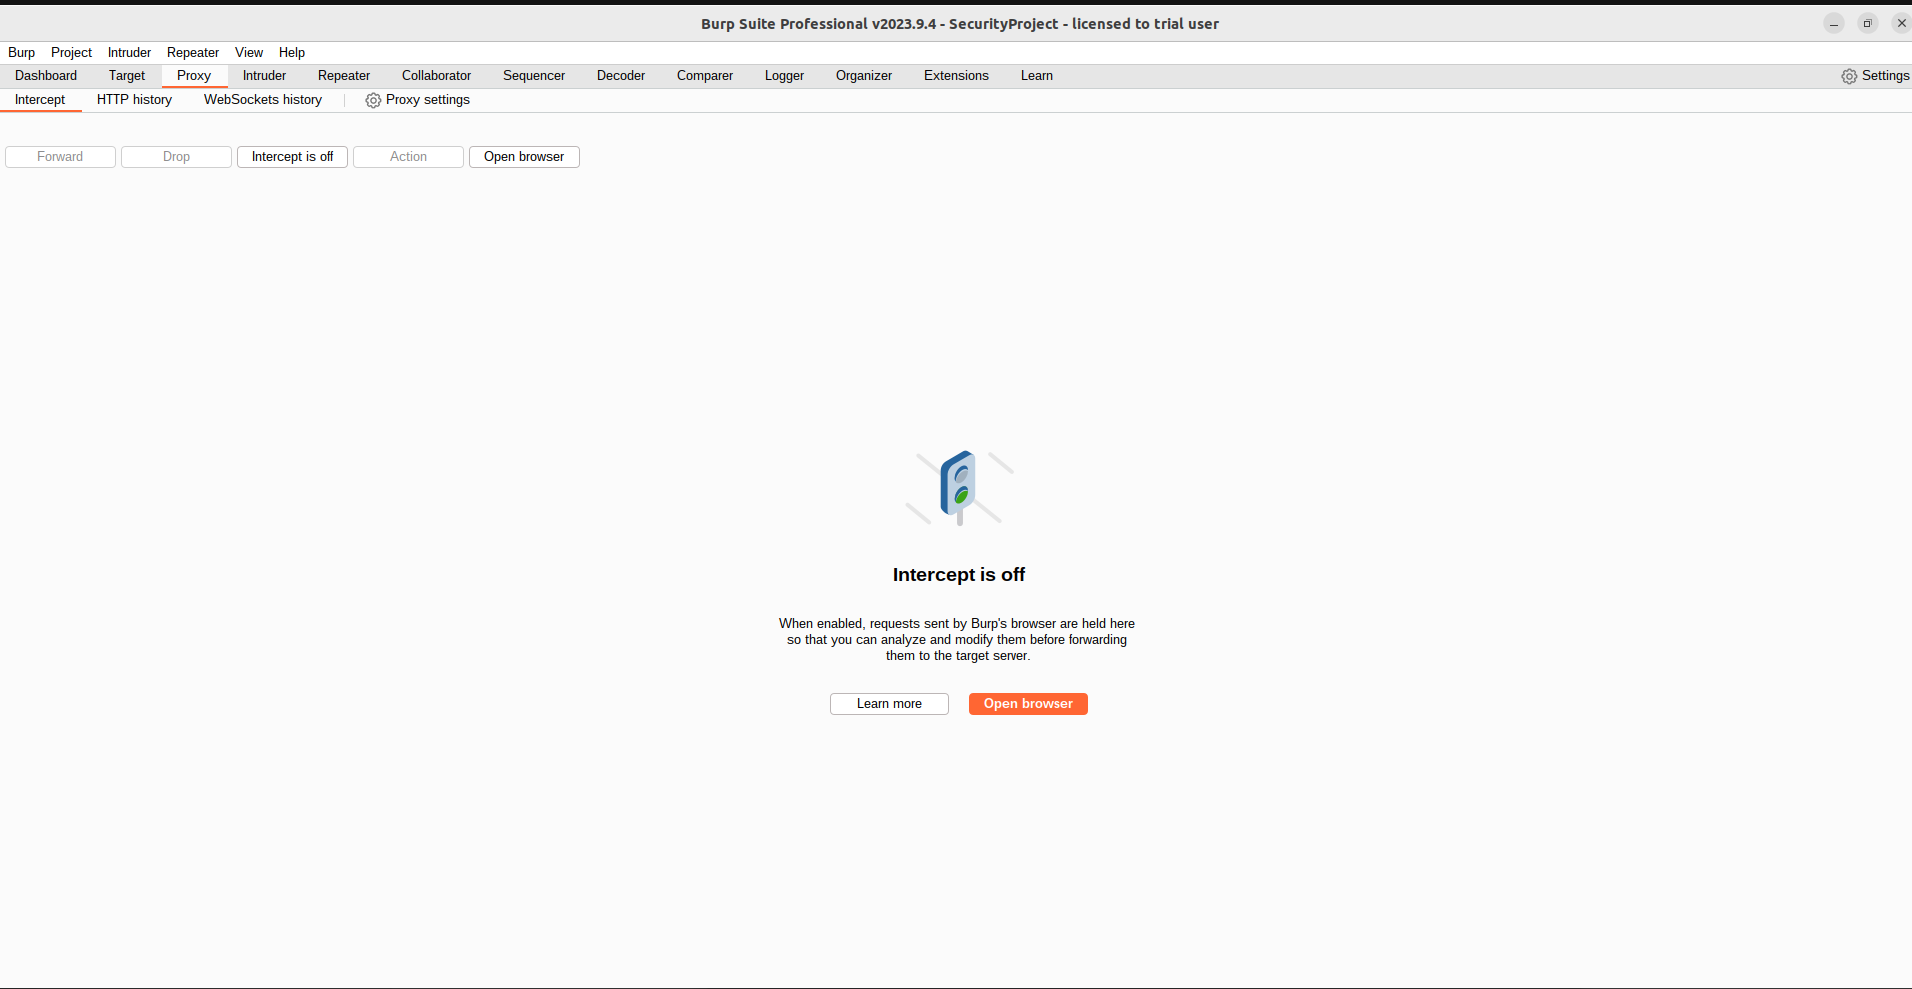
\includegraphics[width=1\textwidth]{Images/anikaScreensots/Proxy1.png}
    \caption{go to proxy tab}
    \label{fig:enter-label}
\end{figure}

\begin{figure}[H]
    \centering
    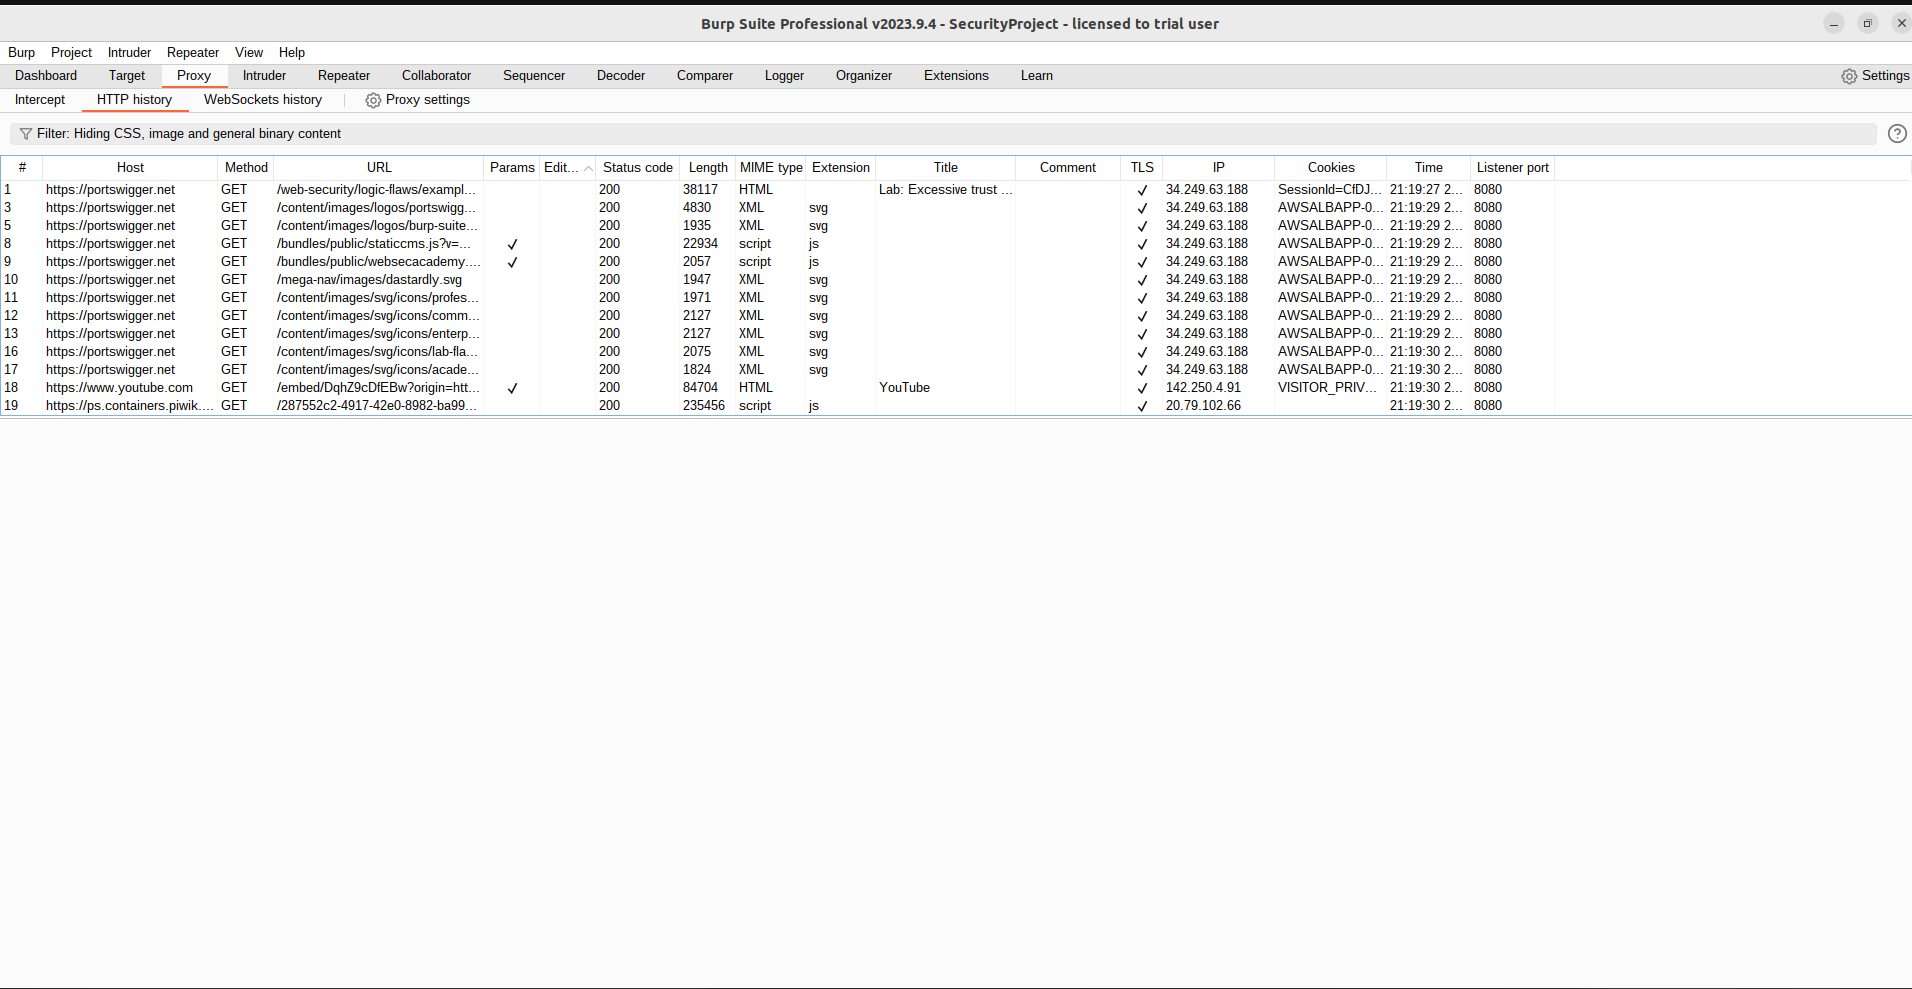
\includegraphics[width=1\textwidth]{Images/anikaScreensots/proxy2.png}
    \caption{examine http history}
    \label{fig:enter-label}
\end{figure}
examine each request in details by by clicking on a request

\begin{figure}[H]
    \centering
    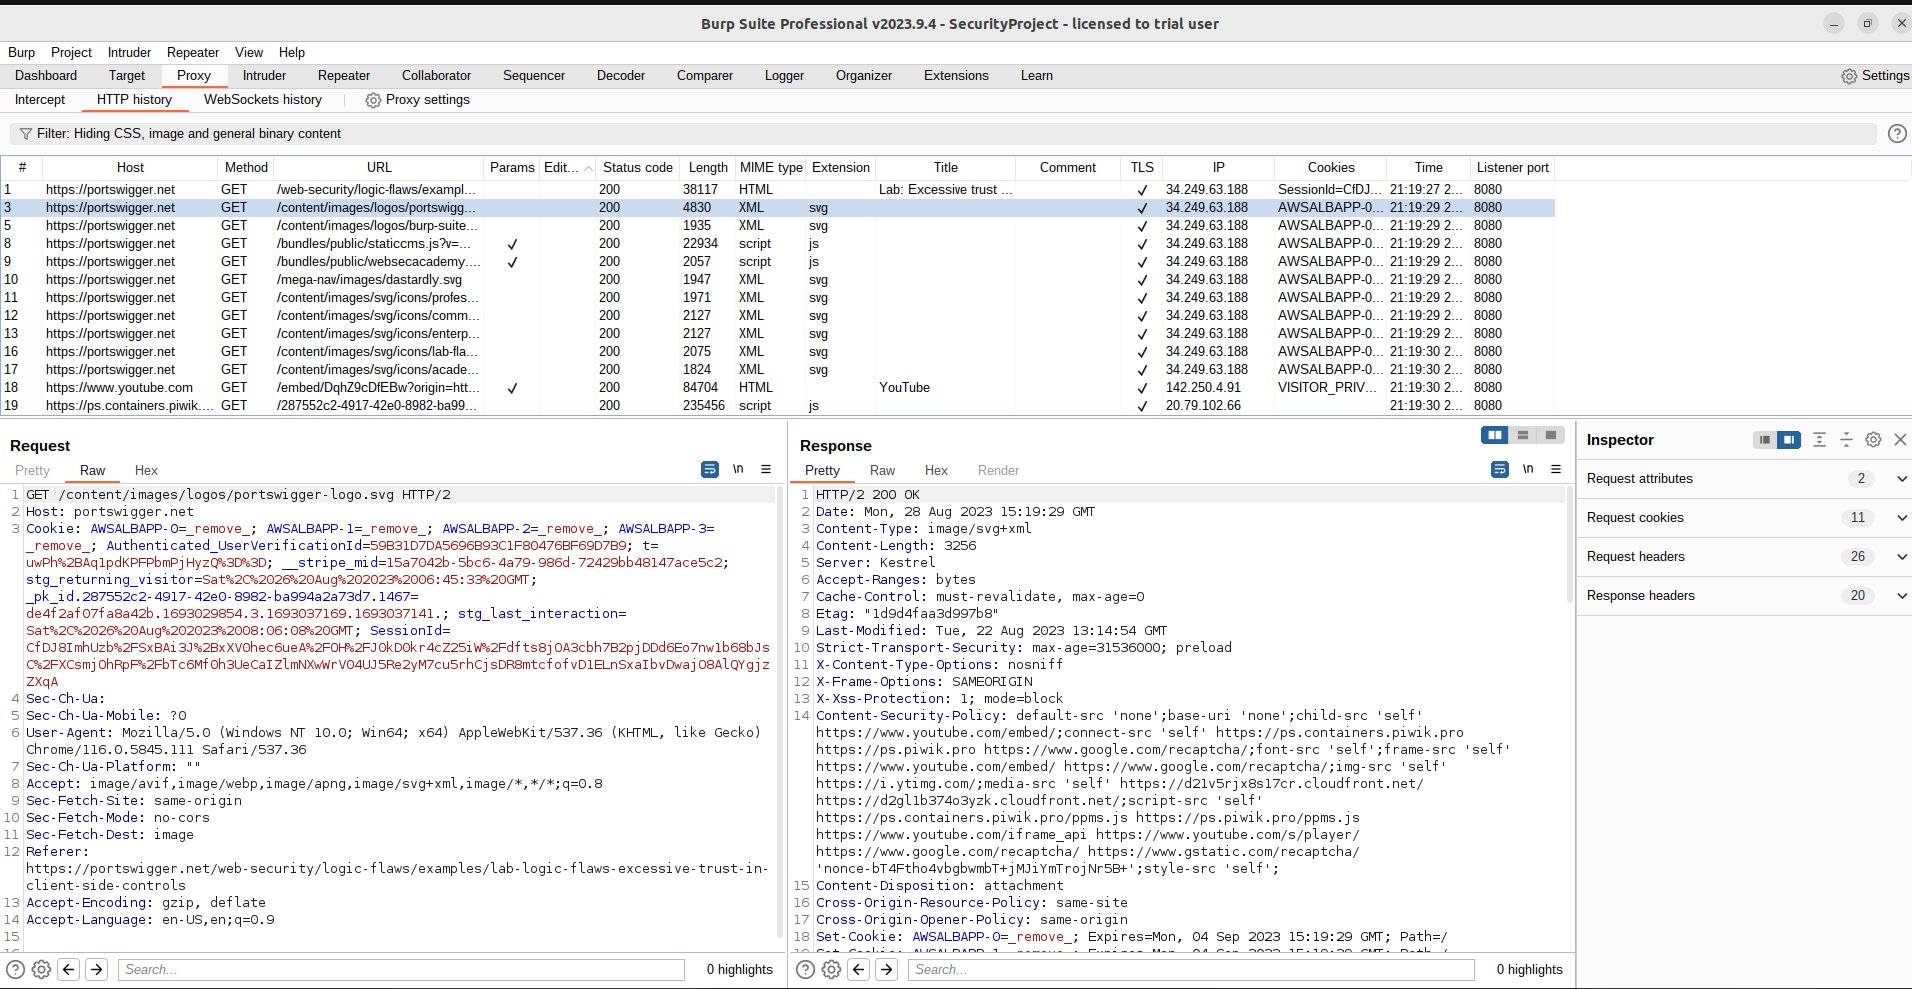
\includegraphics[width=1\textwidth]{Images/anikaScreensots/proxy3.png}
    \caption{examine request}
    \label{fig:enter-label}
\end{figure}



\subsubsection*{Modifying http request with burp proxy}

\begin{fullwidth}
    Burp Proxy lets you intercept HTTP requests and responses sent between Burp's browser and the target server. This enables you to study how the website behaves when you perform different actions. Then we can intercept that request and modify it any way we went
\end{fullwidth}

\subsubsection*{Steps}
\begin{fullwidth}
    

We will use an website that's vulnerable. First we will go the website, add the item we want to buy on cart

\begin{figure}[H]
    \centering
    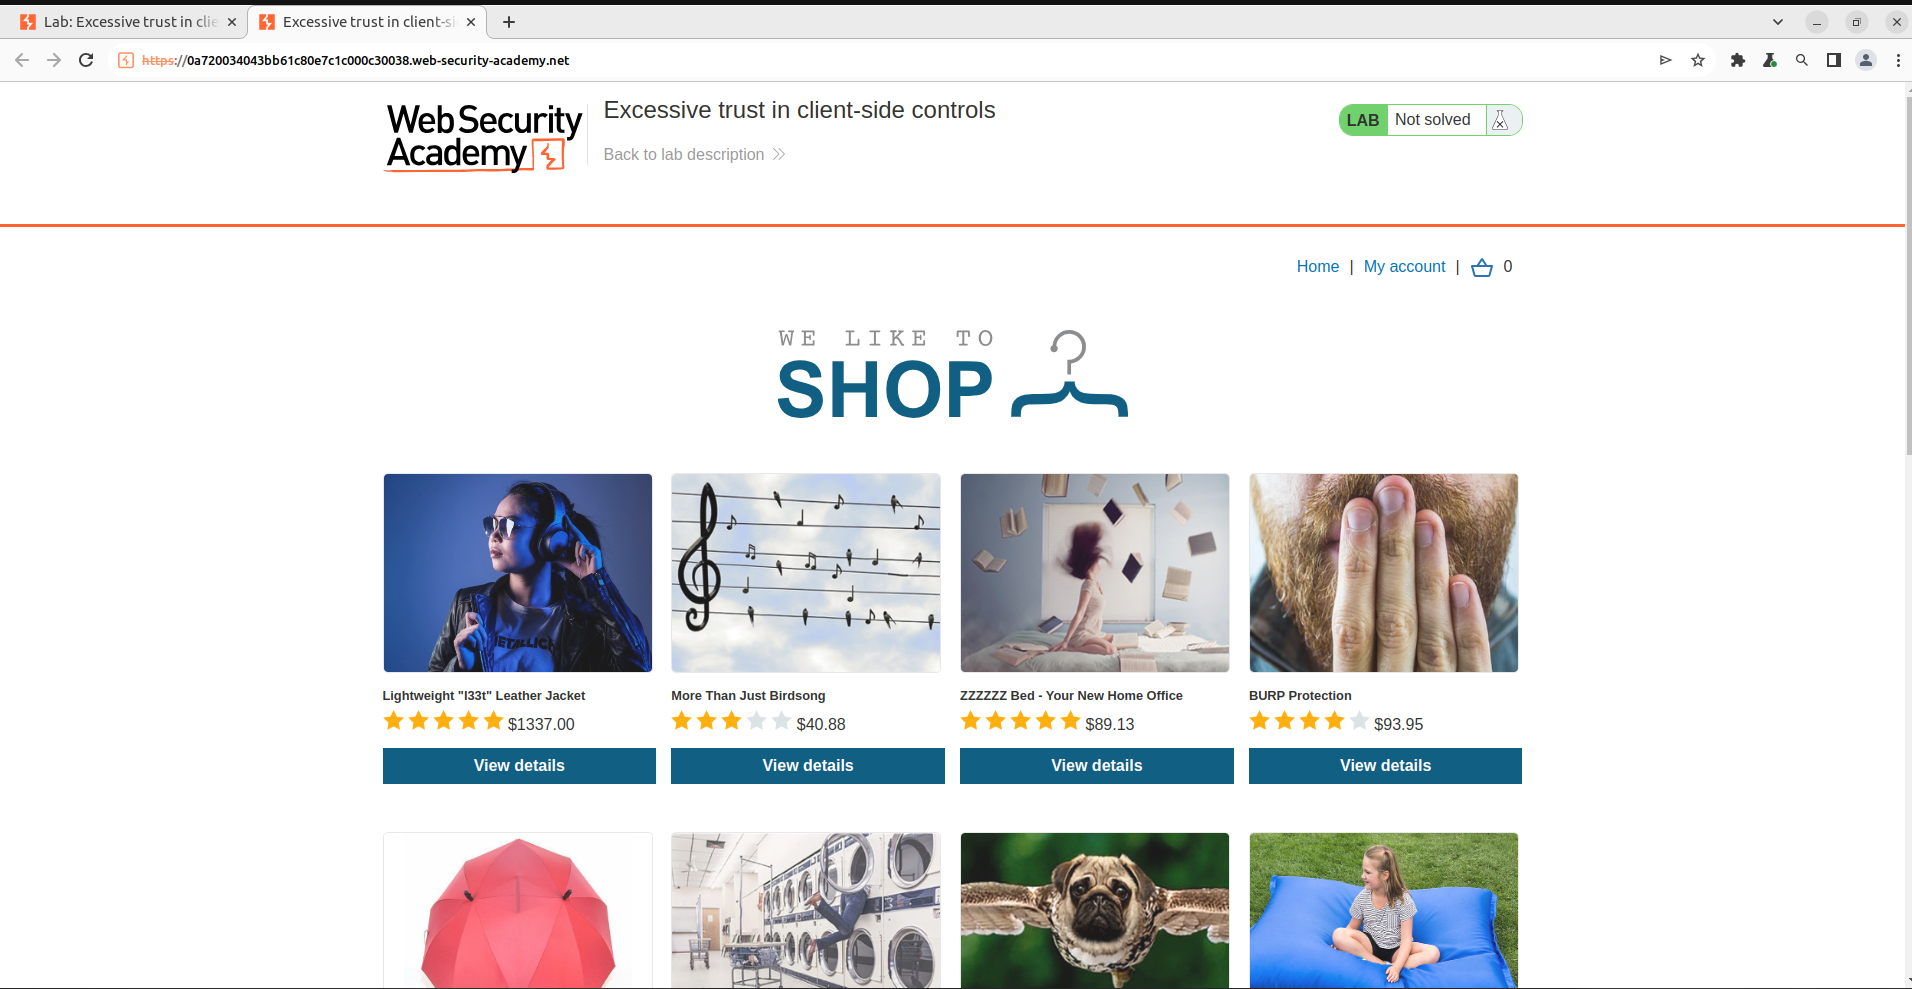
\includegraphics[width=1\textwidth]{Images/anikaScreensots/lab1.png}
    \caption{Caption}
    \label{fig:enter-label}
\end{figure}

\begin{figure}[H]
    \centering
    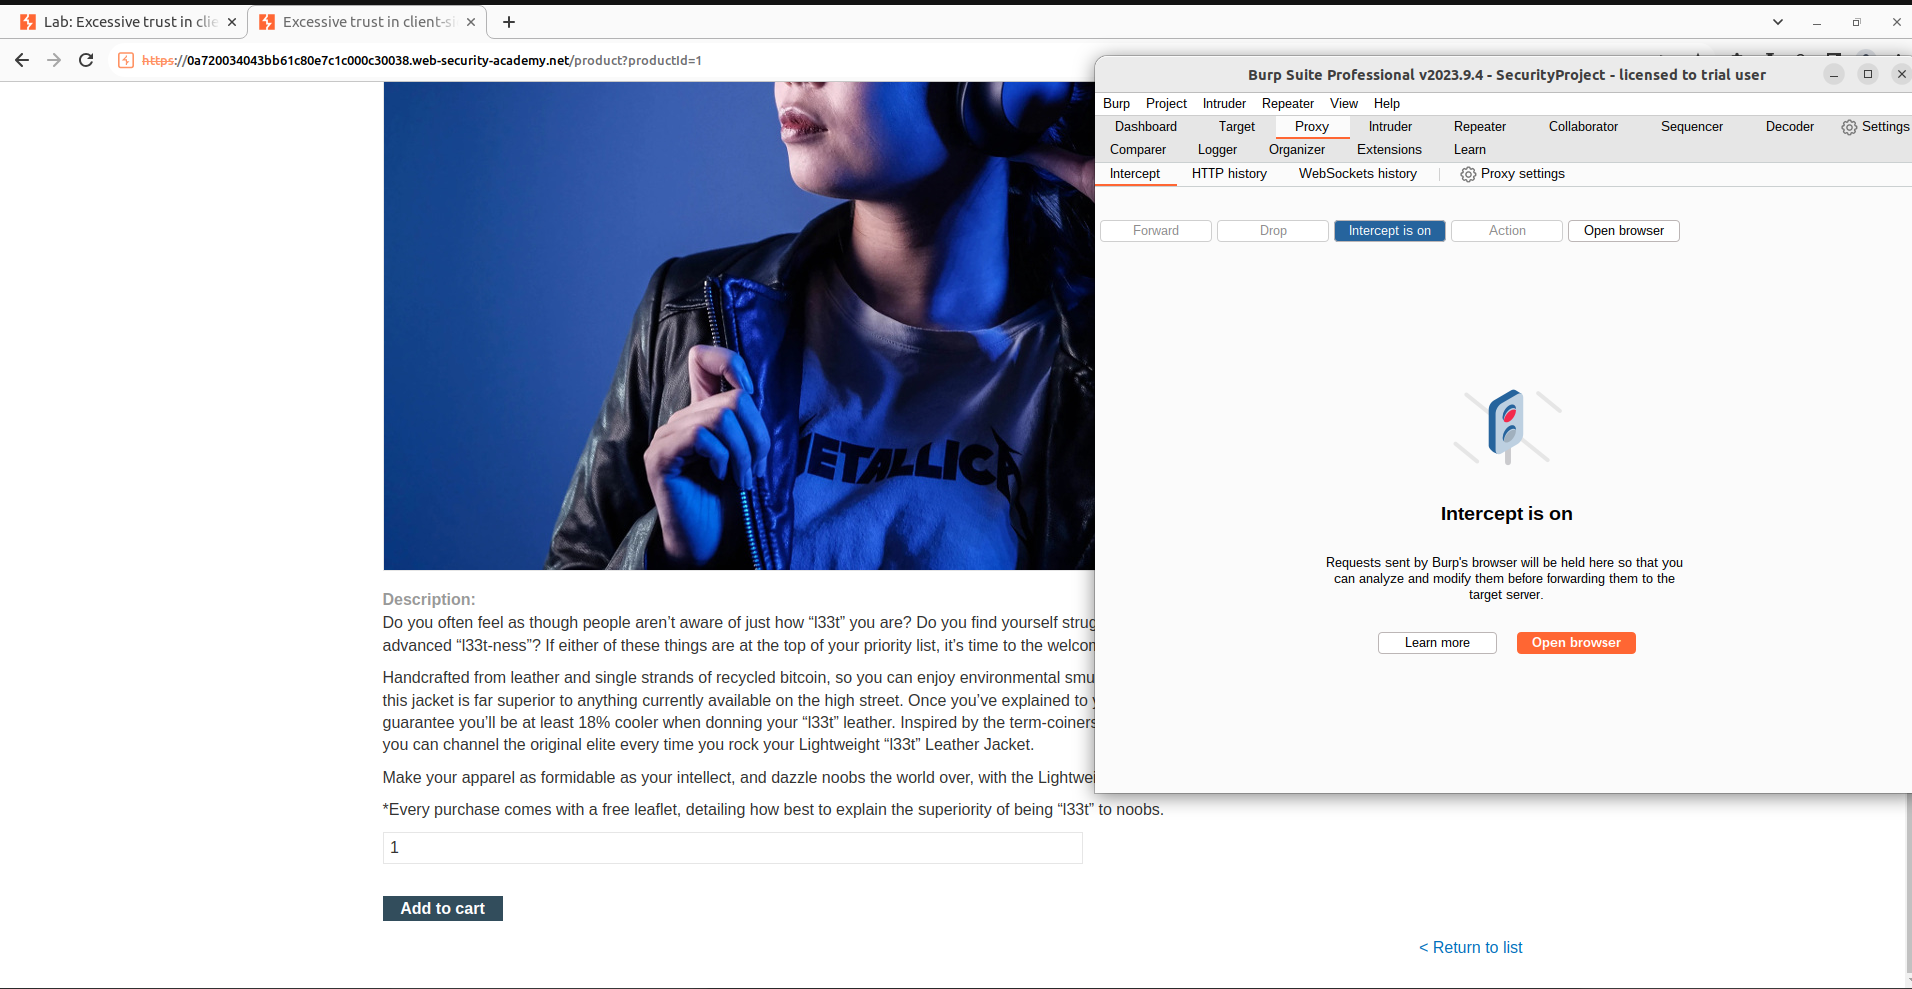
\includegraphics[width=1\textwidth]{Images/anikaScreensots/lab2.png}
    \caption{Caption}
    \label{fig:enter-label}
\end{figure}

we will turn intercept on before clicking on adding to cart and then examine the intercepted request in burp suite.

\begin{figure}[H]
    \centering
    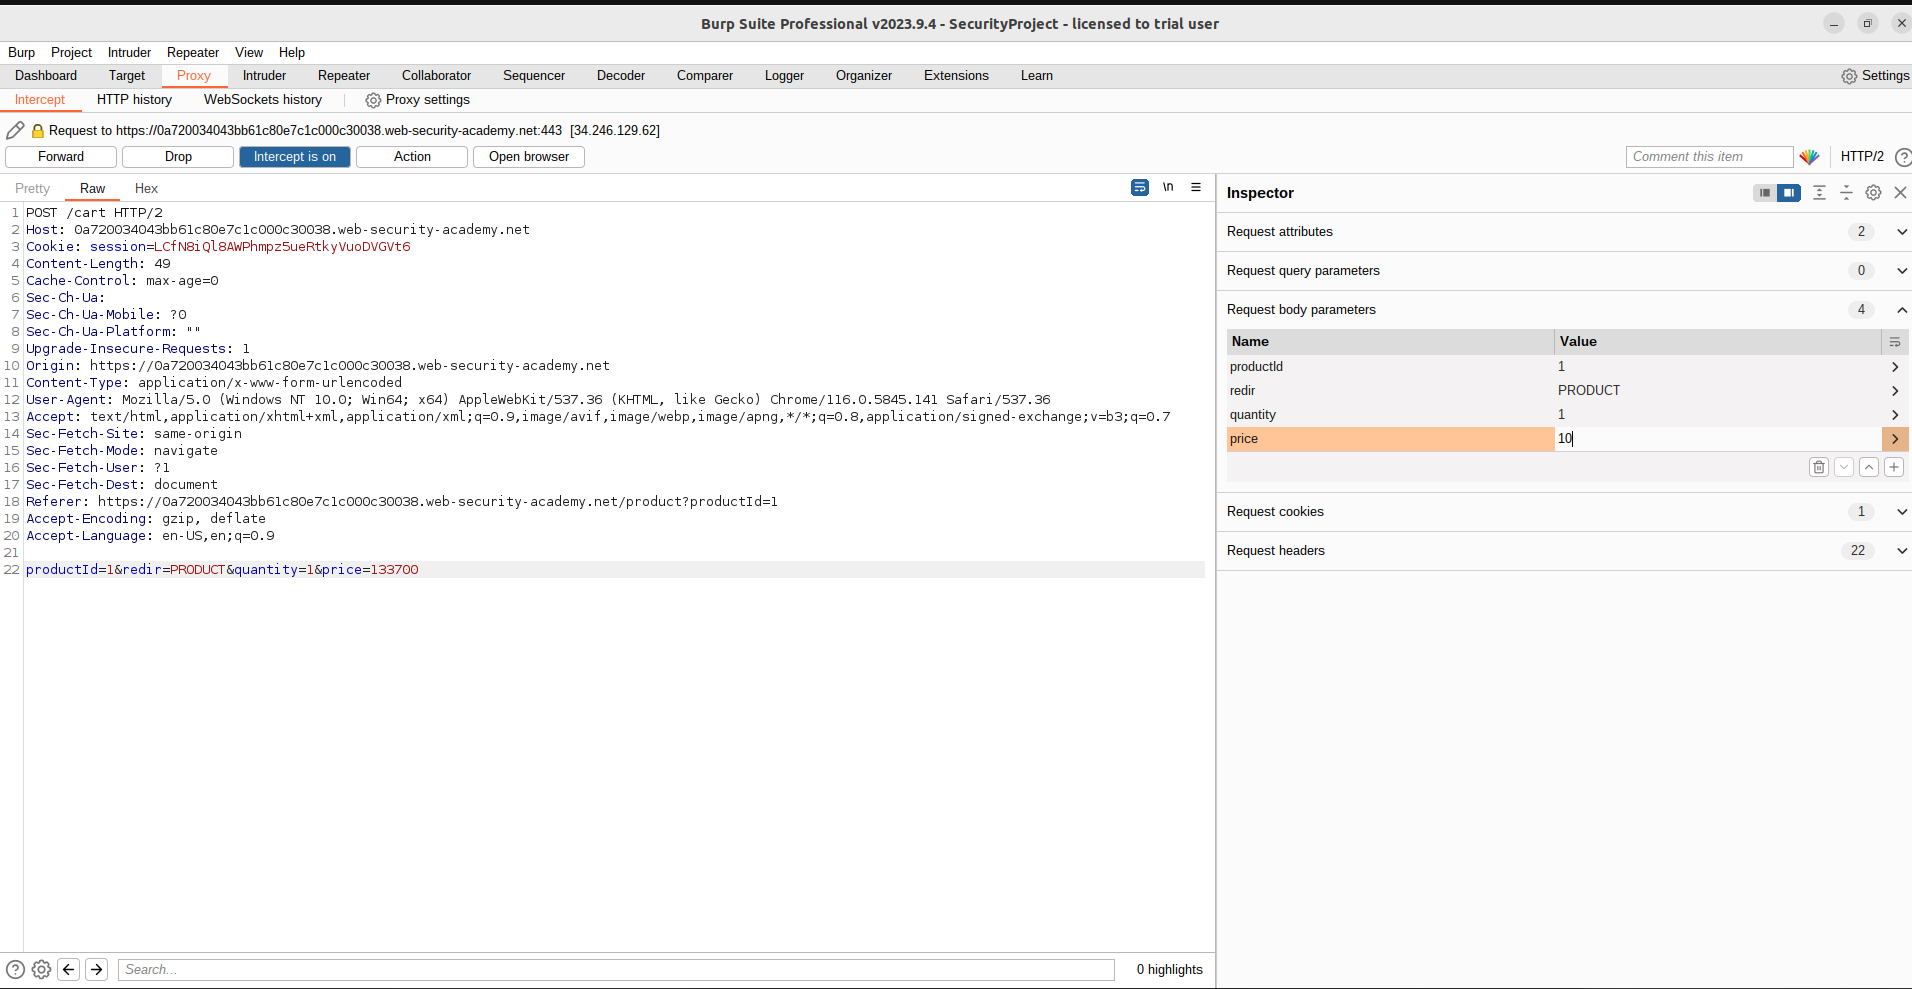
\includegraphics[width=1\textwidth]{Images/anikaScreensots/lab3.png}
    \caption{Caption}
    \label{fig:enter-label}
\end{figure}
We can see that the price and quantity are right there in the http request and we can modify it to change the price value from high to very very low. And then we will forward that request
\begin{figure}[H]
    \centering
    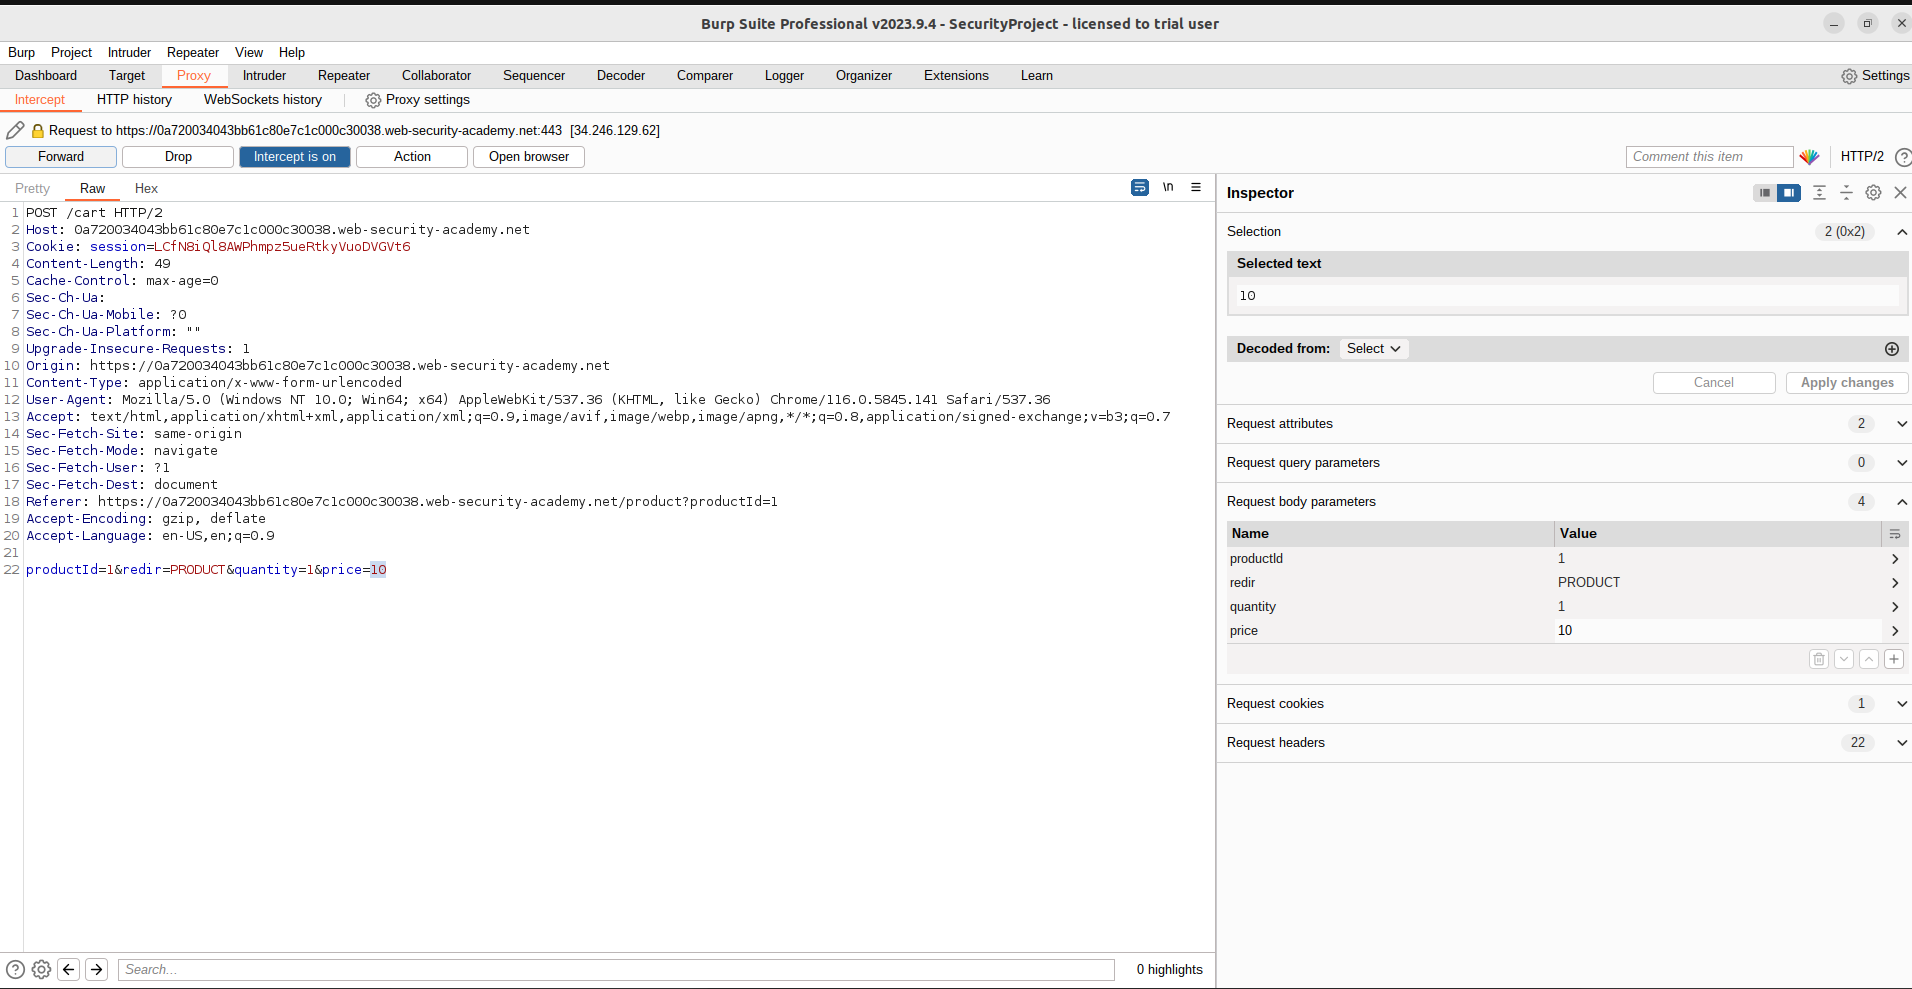
\includegraphics[width=1\textwidth]{Images/anikaScreensots/lab4.png}
    \caption{Caption}
    \label{fig:enter-label}
\end{figure}

we see that in the cart two items have been added to cart significantly below their actual price.
\begin{figure}[H]
    \centering
    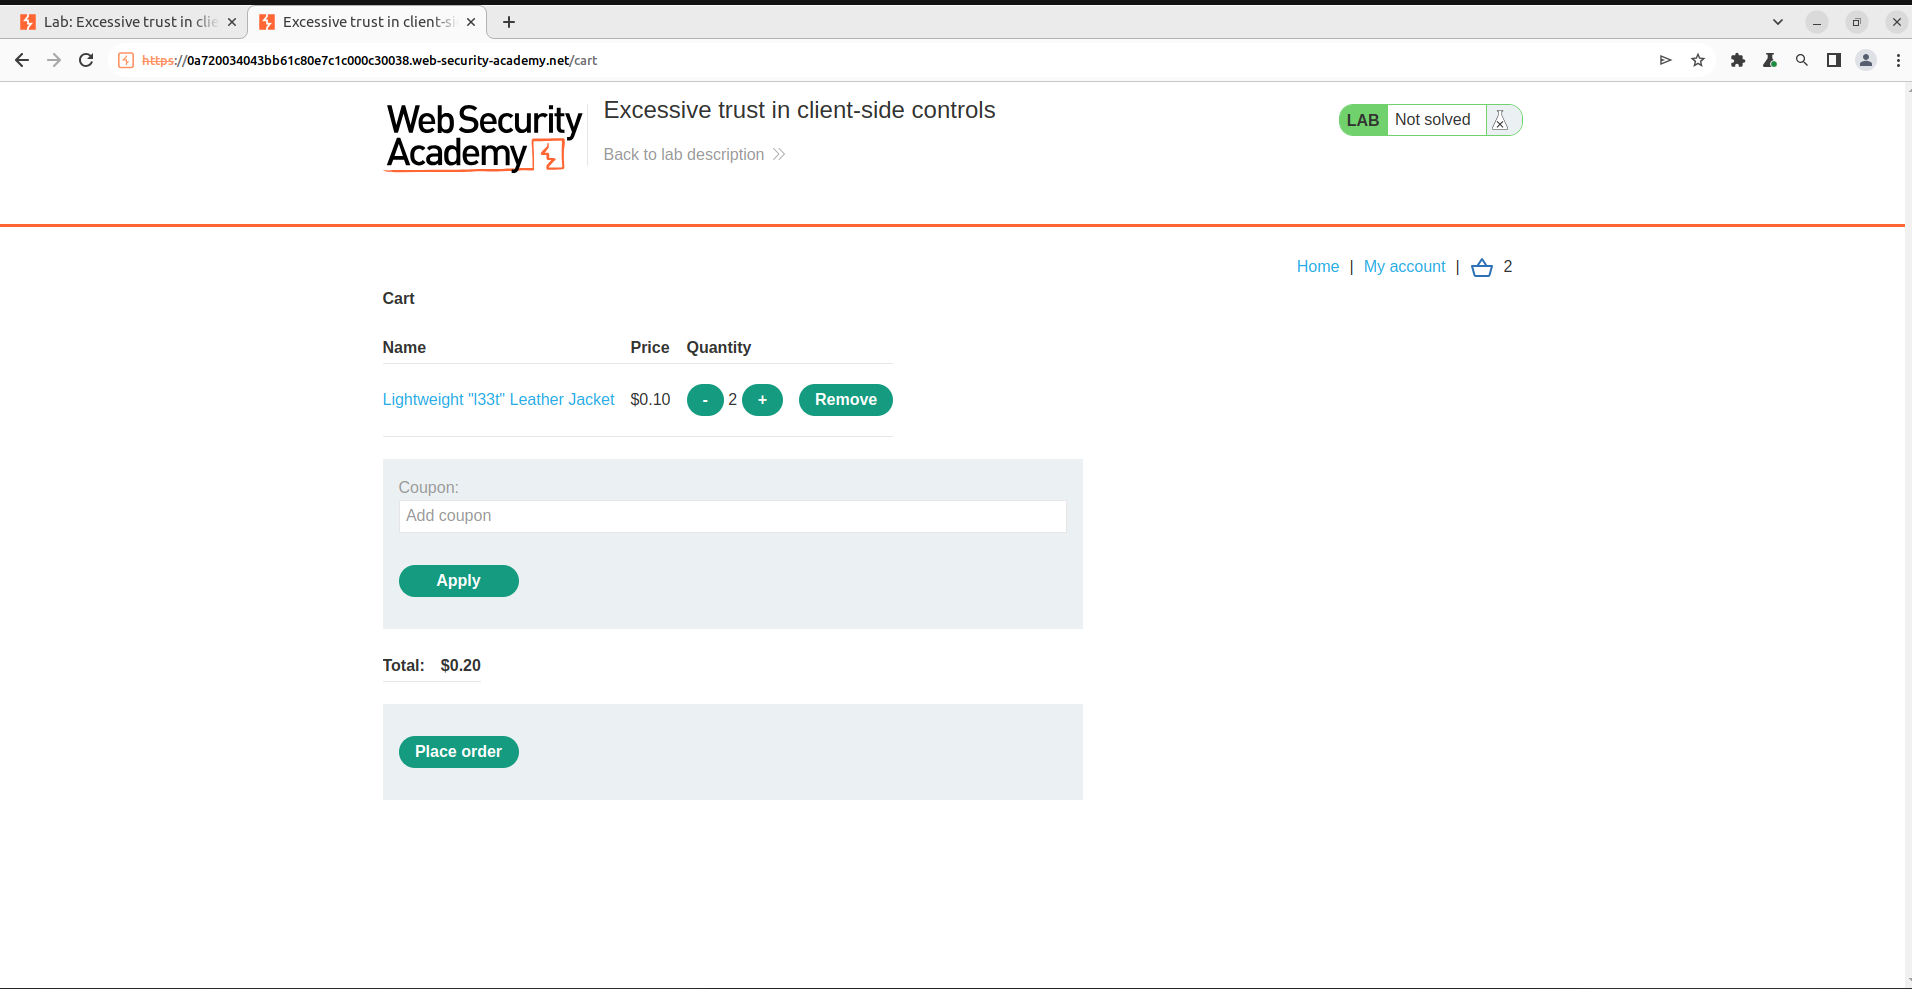
\includegraphics[width=1\textwidth]{Images/anikaScreensots/lab5.png}
    \caption{Caption}
    \label{fig:enter-label}
\end{figure}
\end{fullwidth}

\section{Intruder}

\subsection*{When we use intruder}

\begin{fullwidth}Burp Intruder is a tool for automating customized attacks against web applications. It enables you to configure attacks that send the same HTTP request over and over again, inserting different payloads into predefined positions each time.\end{fullwidth}



\subsection*{Testing authentication mechanism}

\begin{fullwidth}Testing authentication mechanisms using Bu rp Intruder is a crucial step in assessing the security of a web application. Authentication is a critical component that safeguards user accounts and sensitive data. Burp Intruder allows security testers to perform various types of attacks to identify vulnerabilities in the authentication process\end{fullwidth}



\subsection*{Enumerating usernames}

\begin{fullwidth}Using burp intruder, we can enumerate a registration or login form. First we will try to login using a random username and password. Then we will examine the request and send it to burp intruder. Burp intruder will keep sending the request with possible different usernames and passwords. We will check the responses to find out any anomaly with one of the inputs in the hope that it might gain us some information \end{fullwidth}


\subsubsection*{Steps}

To test authentication mechanism we will try to login in to a vulnerable website.

\begin{figure}[H]
    \centering
    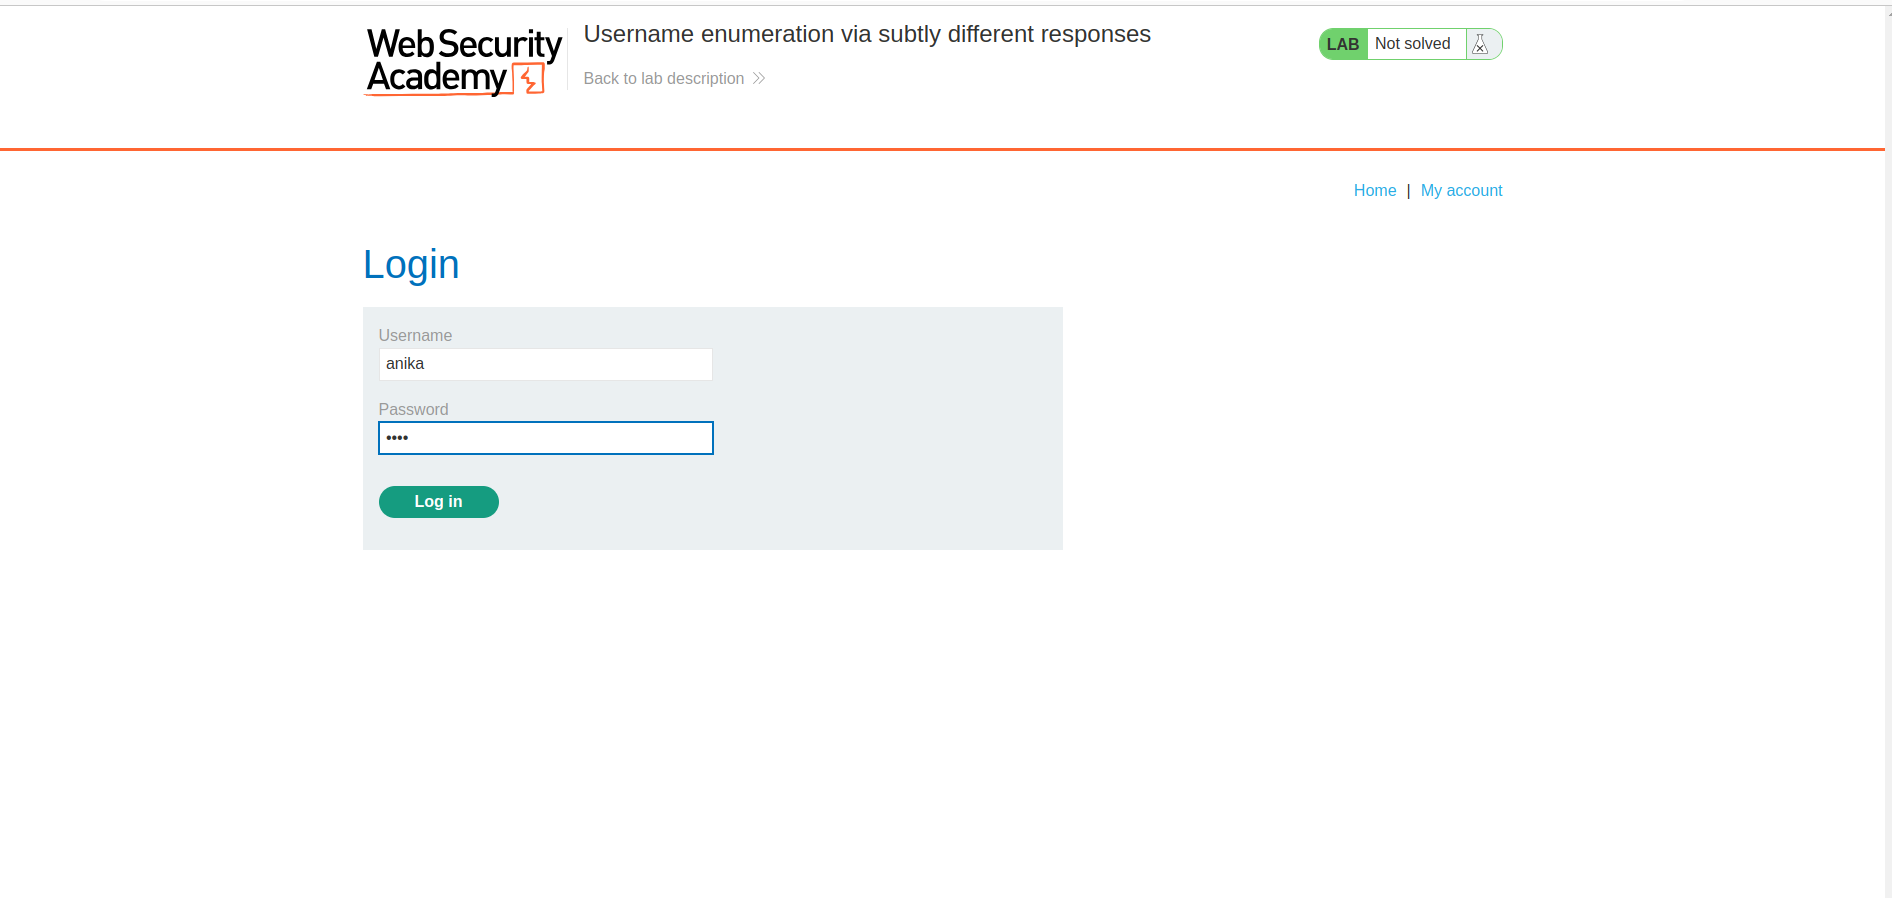
\includegraphics[width=1\textwidth]{Images/anikaScreensots/enumeratinStart.png}
    \caption{trying to login with incorrect usernames and passwords}
    \label{fig:enter-label}
\end{figure}
	

the we will open burp suite and send the request to intruder.   

\begin{figure}[H]
    \centering
    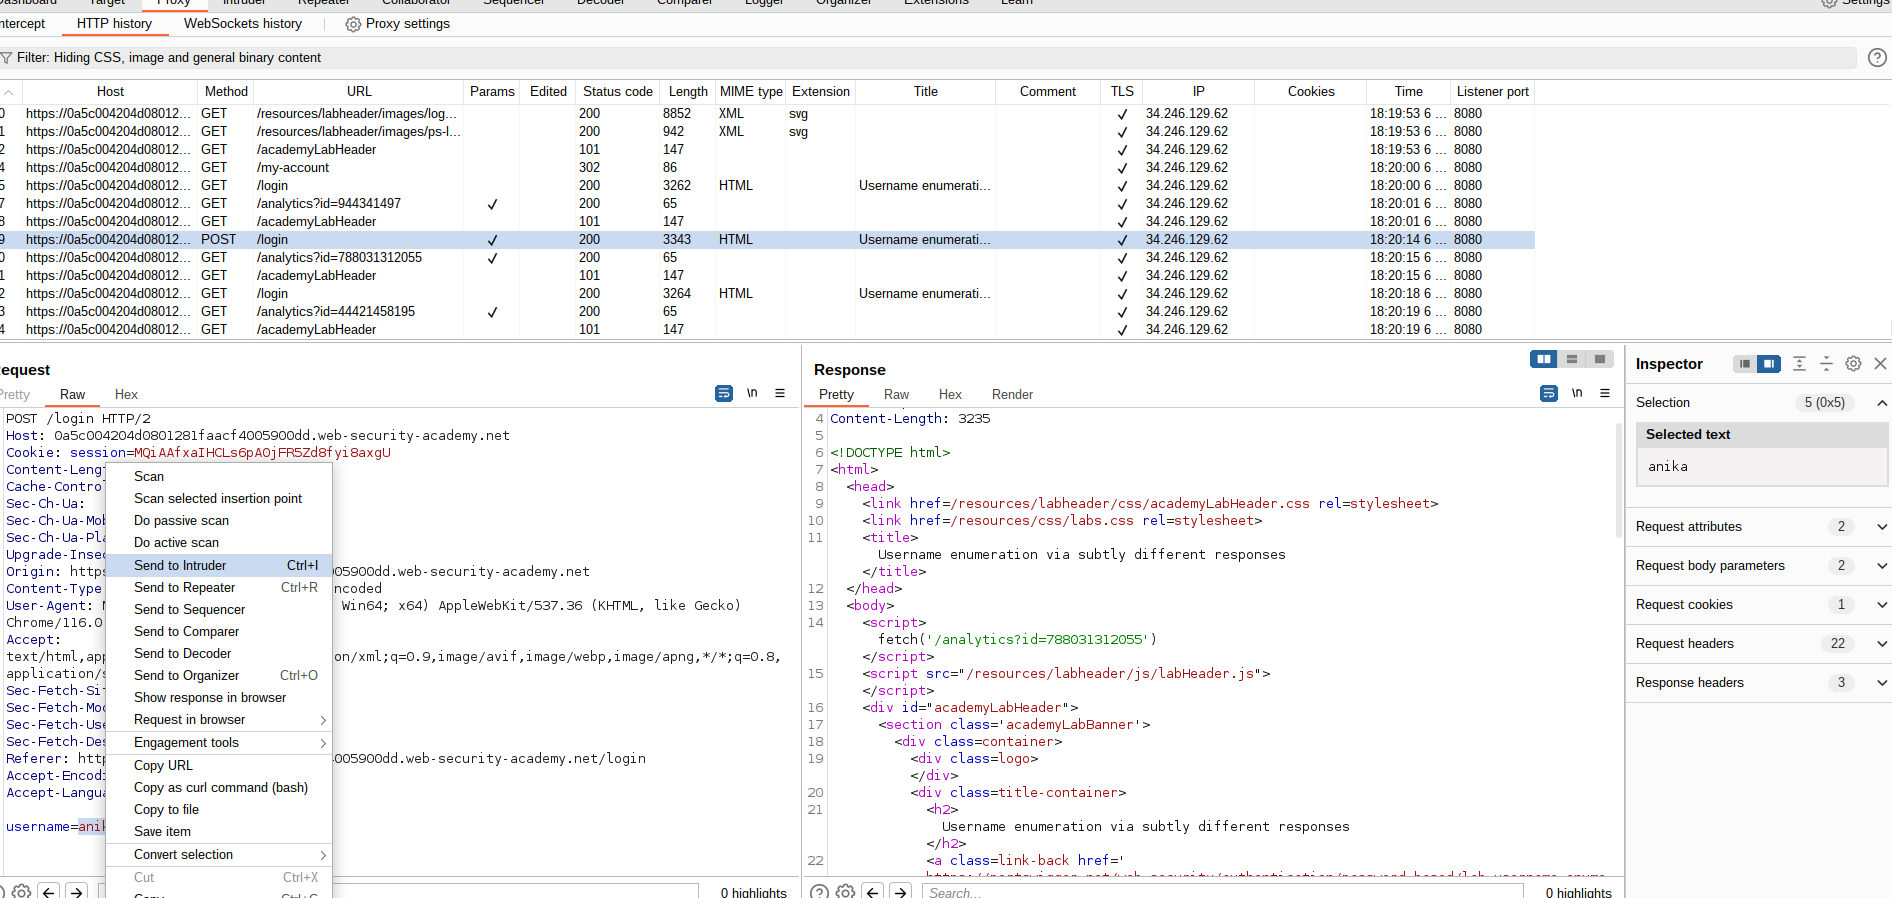
\includegraphics[width=1\textwidth]{Images/anikaScreensots/EnuStep1.png}
    \caption{send the request to intruder}
    \label{fig:enter-label}
\end{figure}

\begin{figure}[H]
    \centering
    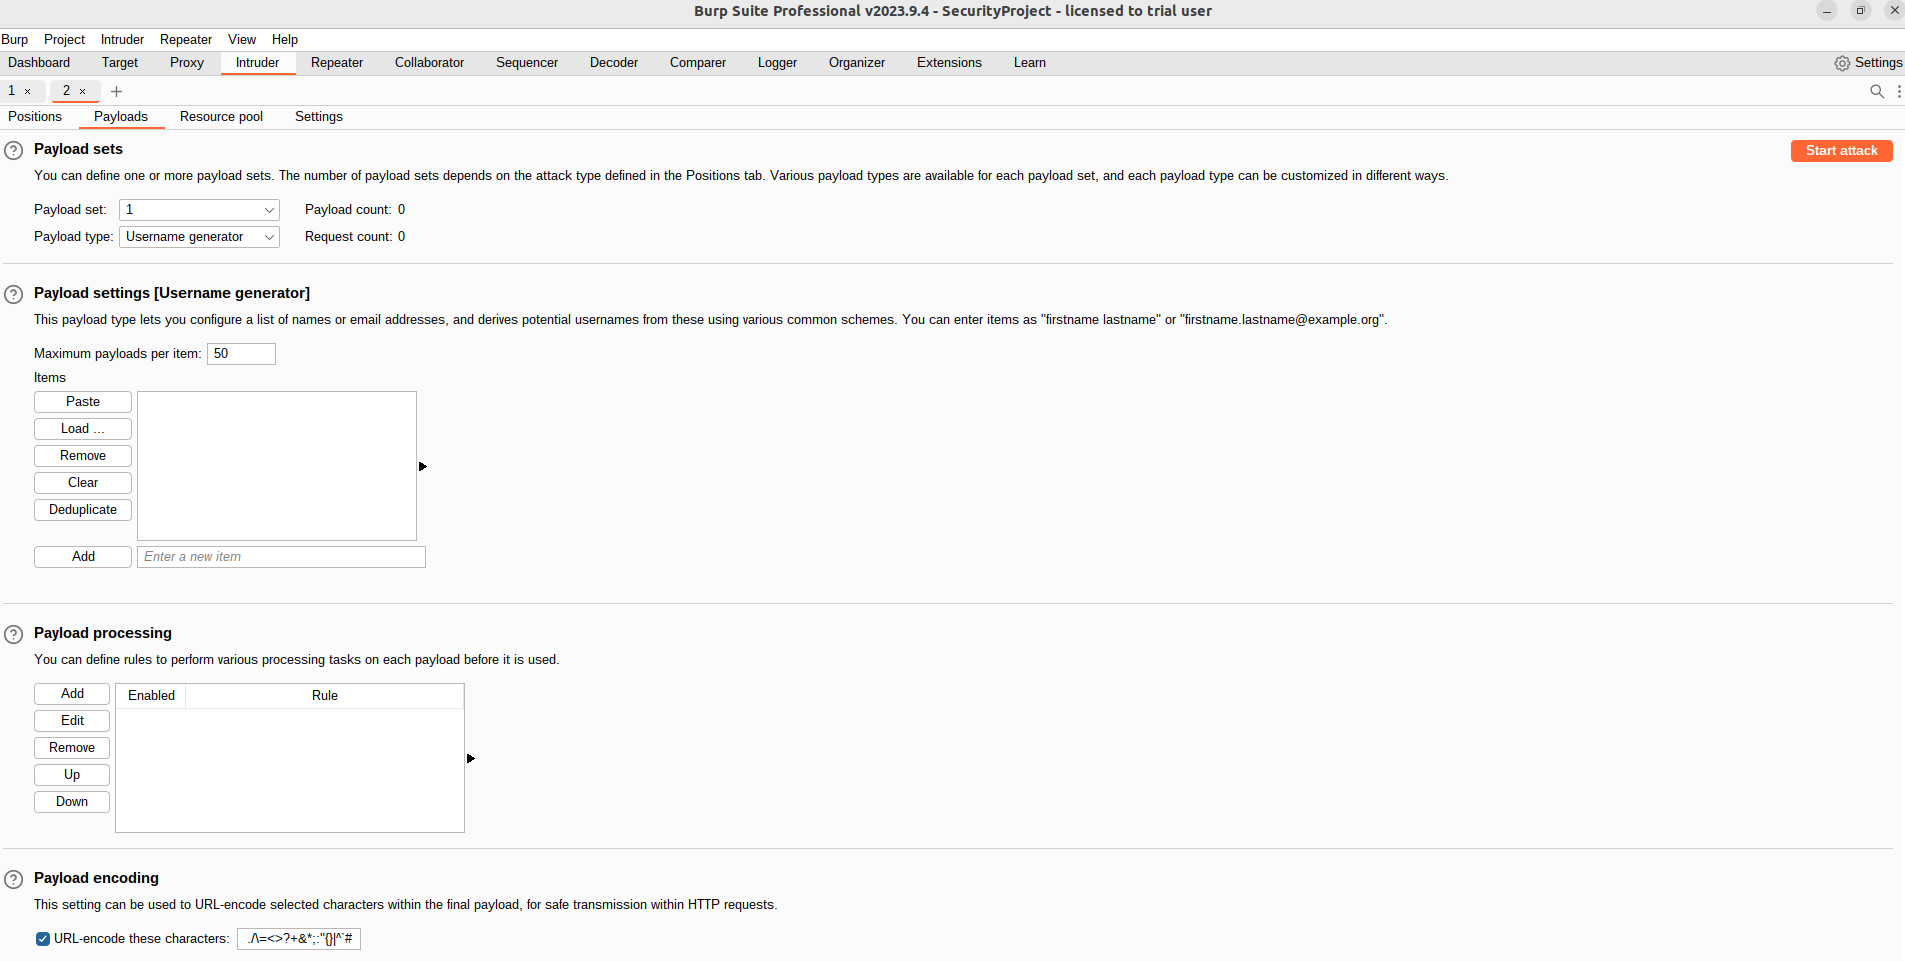
\includegraphics[width=1\textwidth]{Images/anikaScreensots/STEP2.png}
    \caption{setting the payload}
    \label{fig:enter-label}
\end{figure}


 

and click on start attack.

%----------------------------------------------------------------------------------------
%	QUOTATIONS
%----------------------------------------------------------------------------------------

\subsection*{Guessing usernames}

\begin{fullwidth}If we know an user, we can use that name to generate user names based on that knowledge. From the payload type we will use username generator – we can enter the number of usernames we ] want Burp to generate into the maximum payloads per item. For exam, if we know that the name of the attacker is anika monir- burp can generate monir.anika, anikamonir,  \text{anika_monir} and so on.
\end{fullwidth}

\begin{figure}[H]
    \centering
    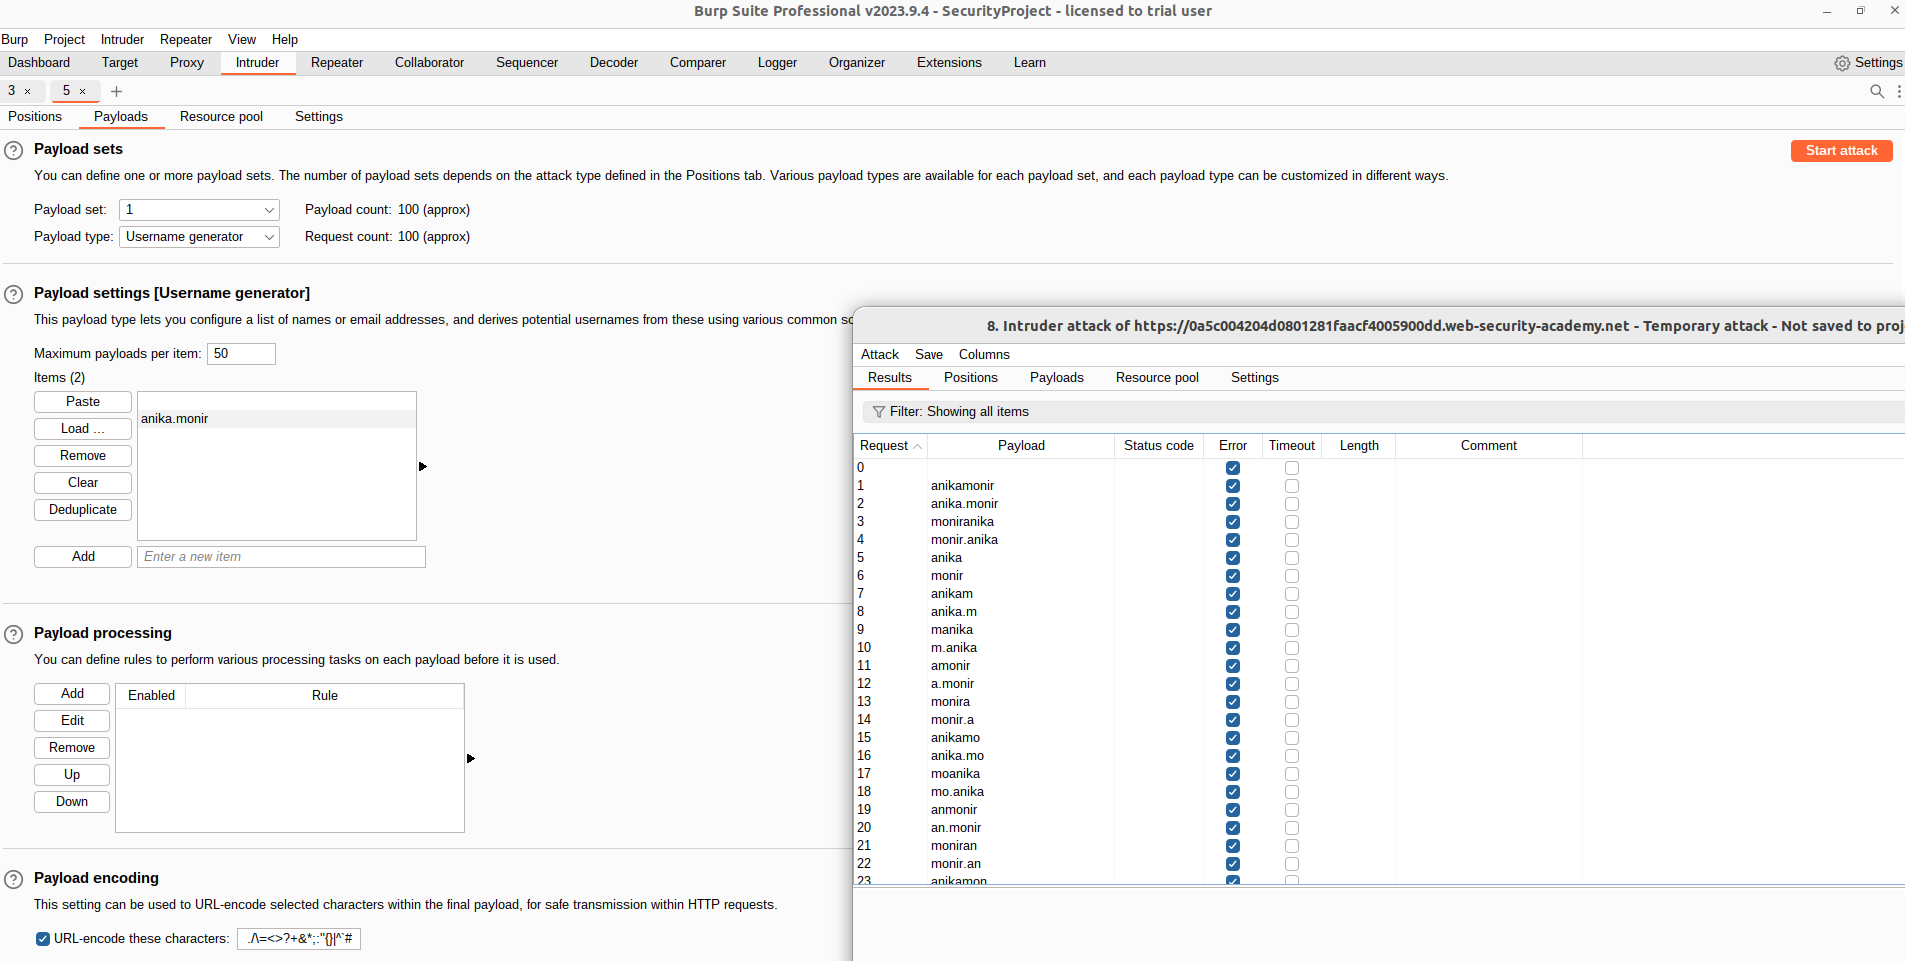
\includegraphics[width=1\textwidth]{Images/anikaScreensots/username.png}
    \caption{implementing the username generator}
    \label{fig:enter-label}
\end{figure}

\subsection*{Brute Forcing Password}
\subsubsection*{Dictionary Attack}
\begin{fullwidth}
    For dictionary attack- We need to make sure that we know at least one valid username. Then we will use a potential list of passwords that we may have gained from previous breach attacks.For example, let’s say we know one username is weiner. Now we will possible passwords from burp suite known password list

\begin{figure}[H]
    \centering
    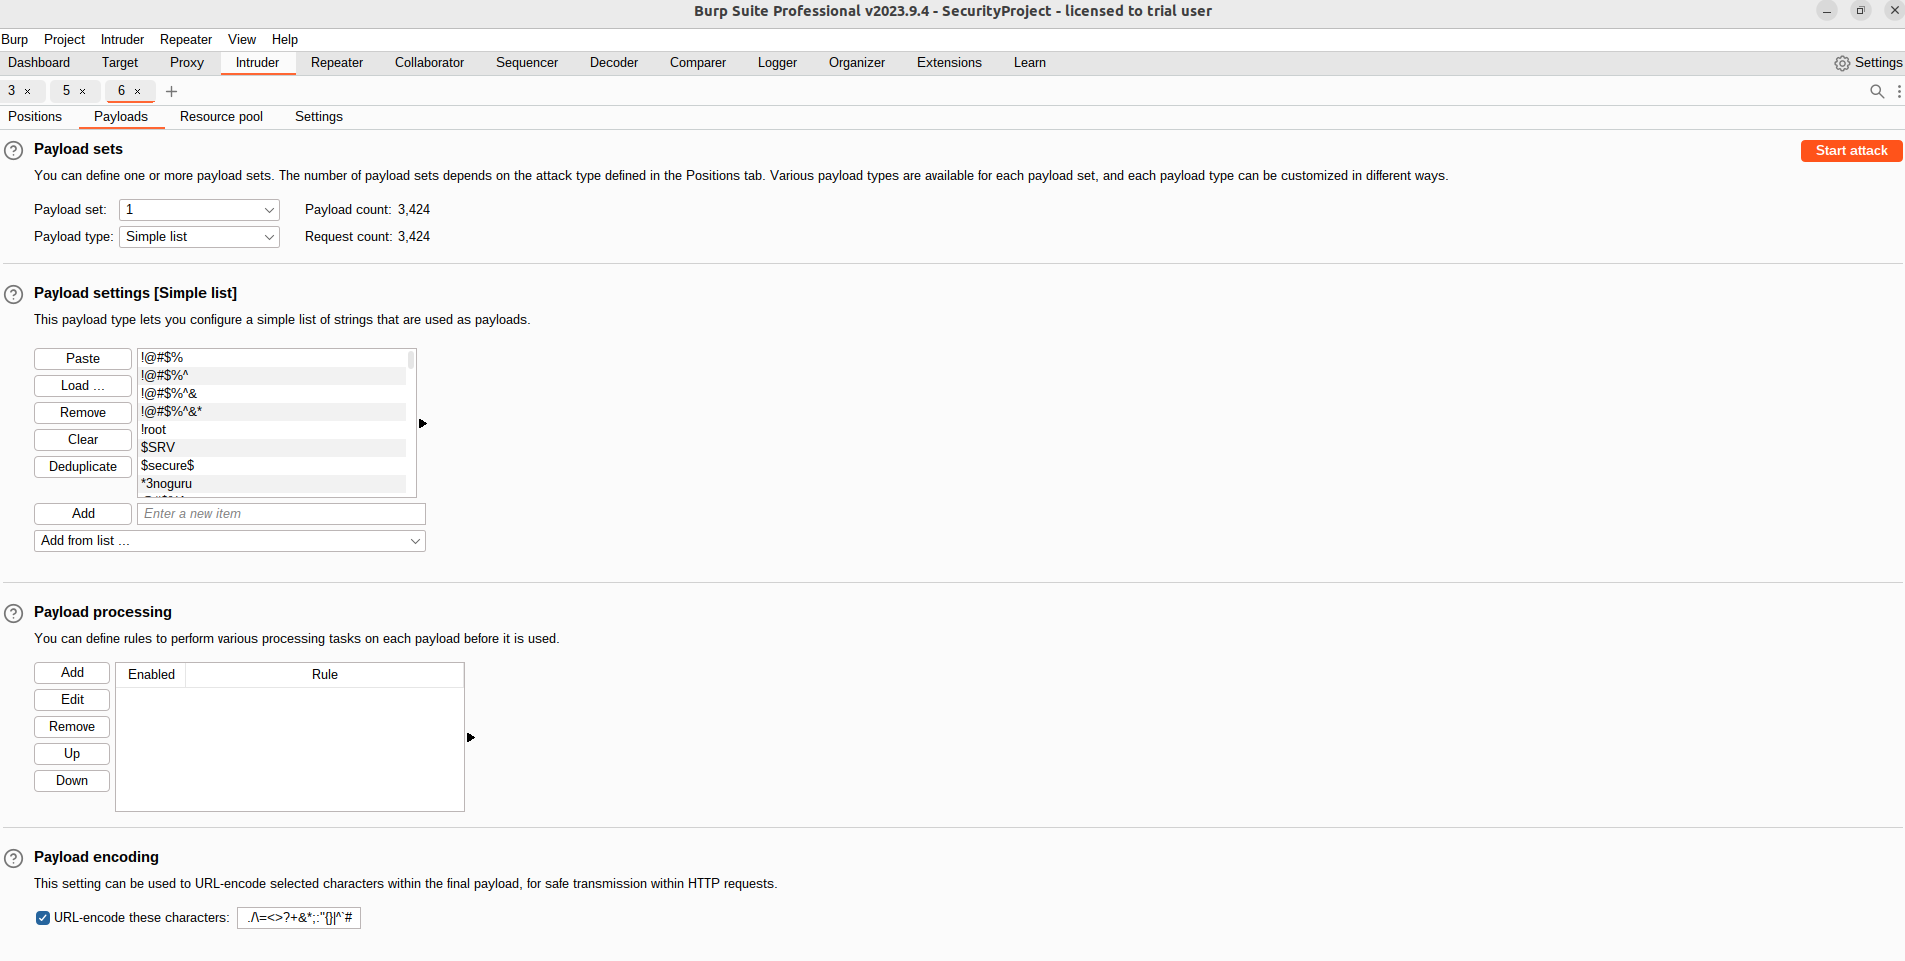
\includegraphics[width=1\textwidth]{Images/anikaScreensots/dictionary1.png}
    \caption{setting the payload a list of known passwords}
    \label{fig:enter-label}
\end{figure}

\begin{figure}[H]
    \centering
    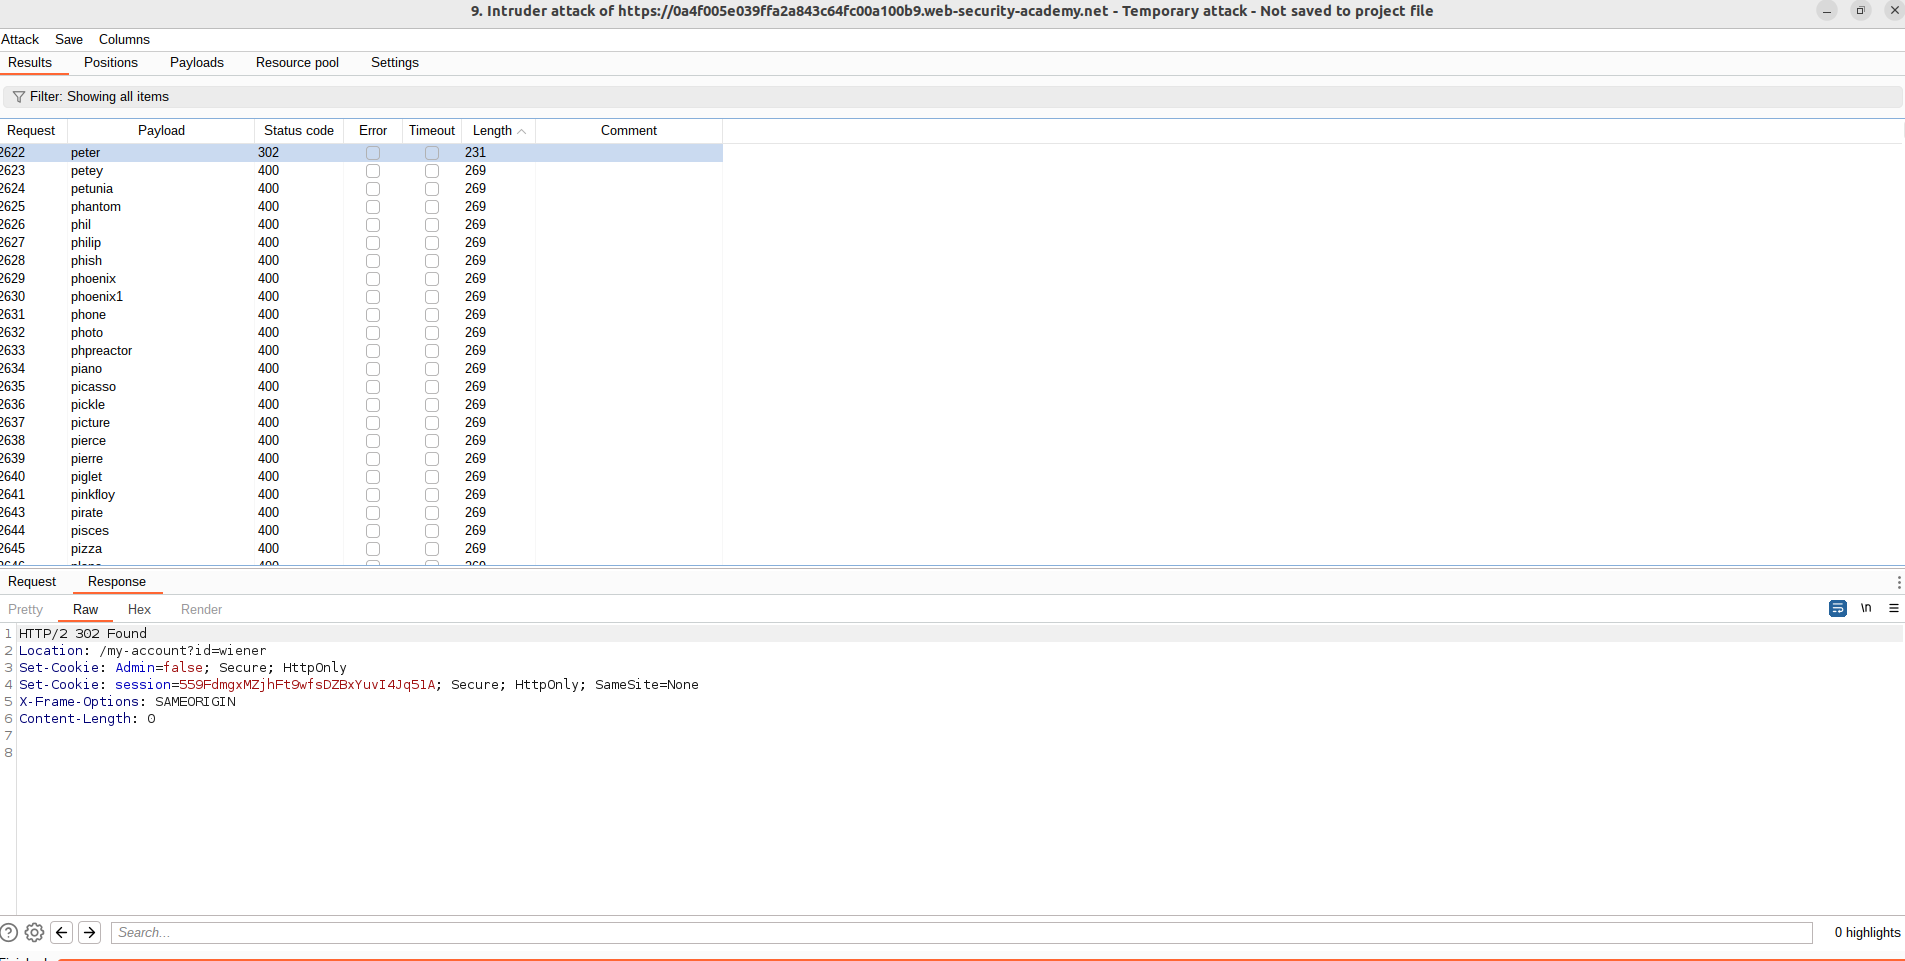
\includegraphics[width=1\textwidth]{Images/anikaScreensots/dictionary2.png}
    \caption{checking the status for different request}
    \label{fig:enter-label}
\end{figure}



\end{fullwidth}
\subsubsection*{Exhaustive Brute Force Attack}
\begin{fullwidth}
    Here we will try every possible combination of character set. This way we will even be able to check for passwords that is uncommon. But we still still need a username that’s valid. Here we can enter the full character set and set the minimum and maximum password length that we want to test for.

    \begin{figure}[H]
    \centering
    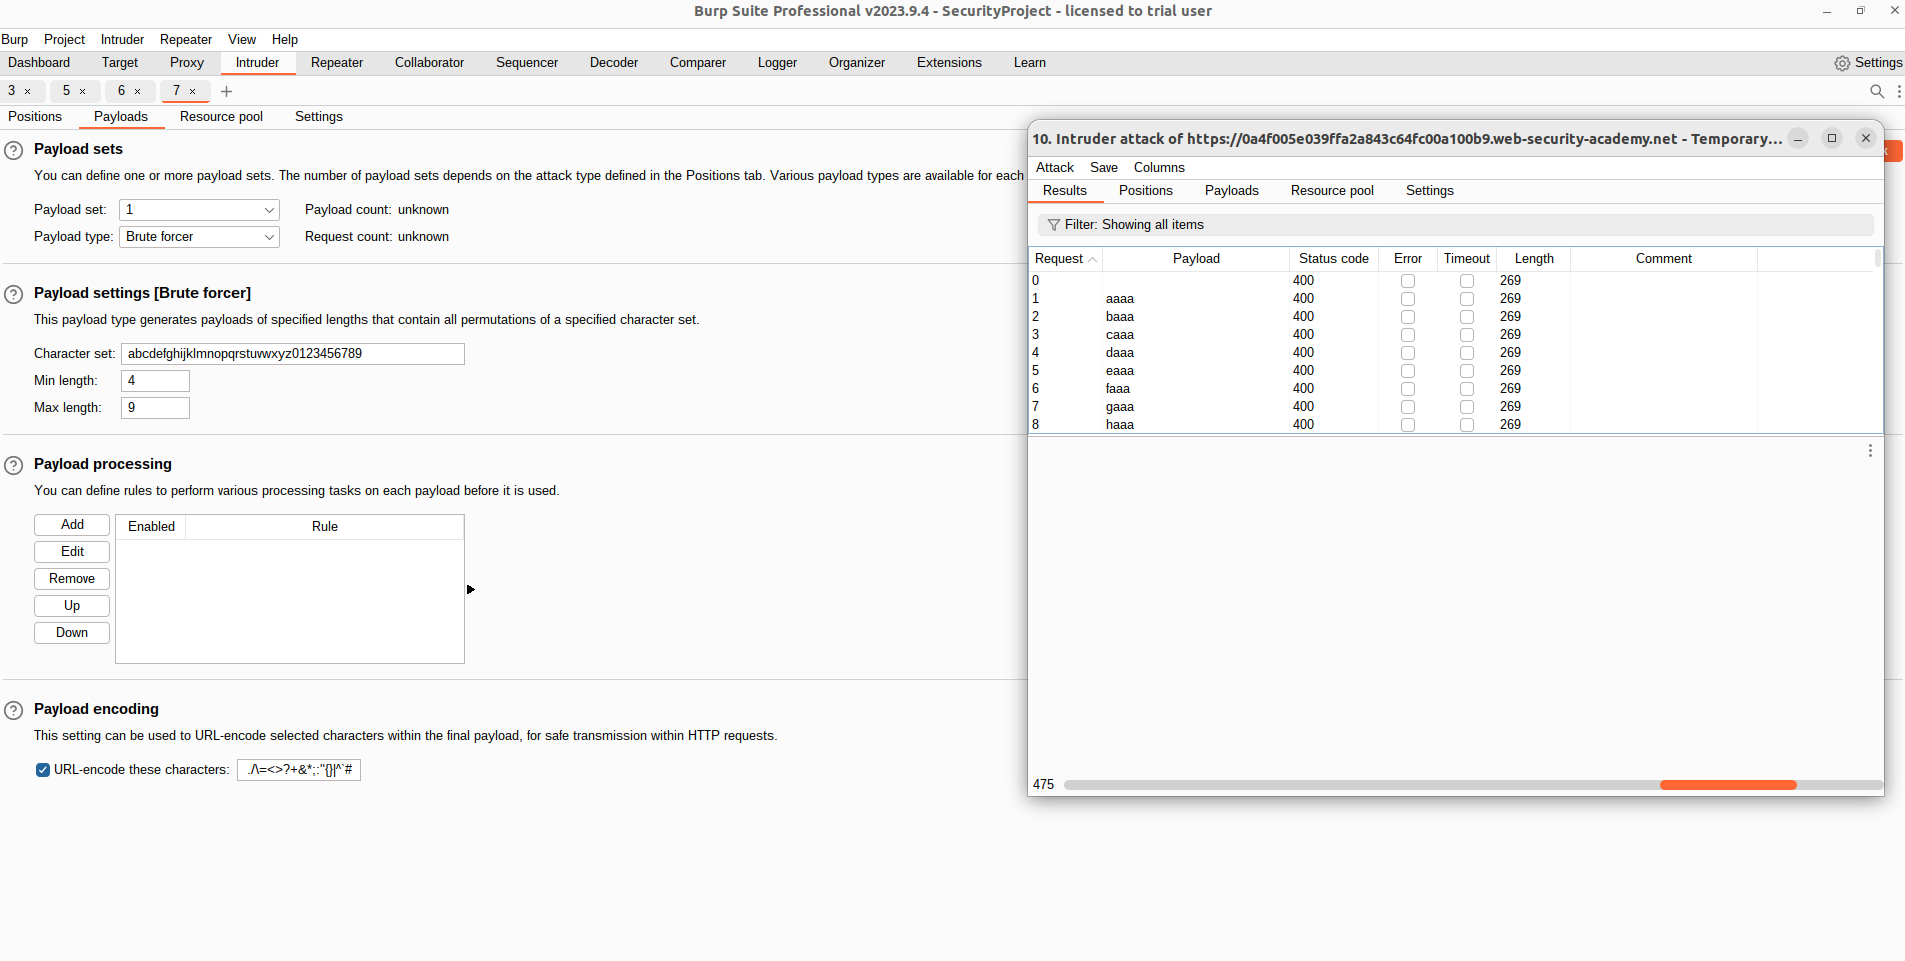
\includegraphics[width=1\textwidth]{Images/anikaScreensots/exaustiveBruteForce.png}
    \caption{}
    \label{fig:enter-label}
\end{figure}
\end{fullwidth}






\subsection*{Credential Stuffing}
\begin{fullwidth}
    Here we use known possible usernames and passwords from websites. This knowledge is usually built up over time from previous breaches. For this we will use the intruder tool and the pitchfork attack type.

    
 \begin{figure}[H]
    \centering
    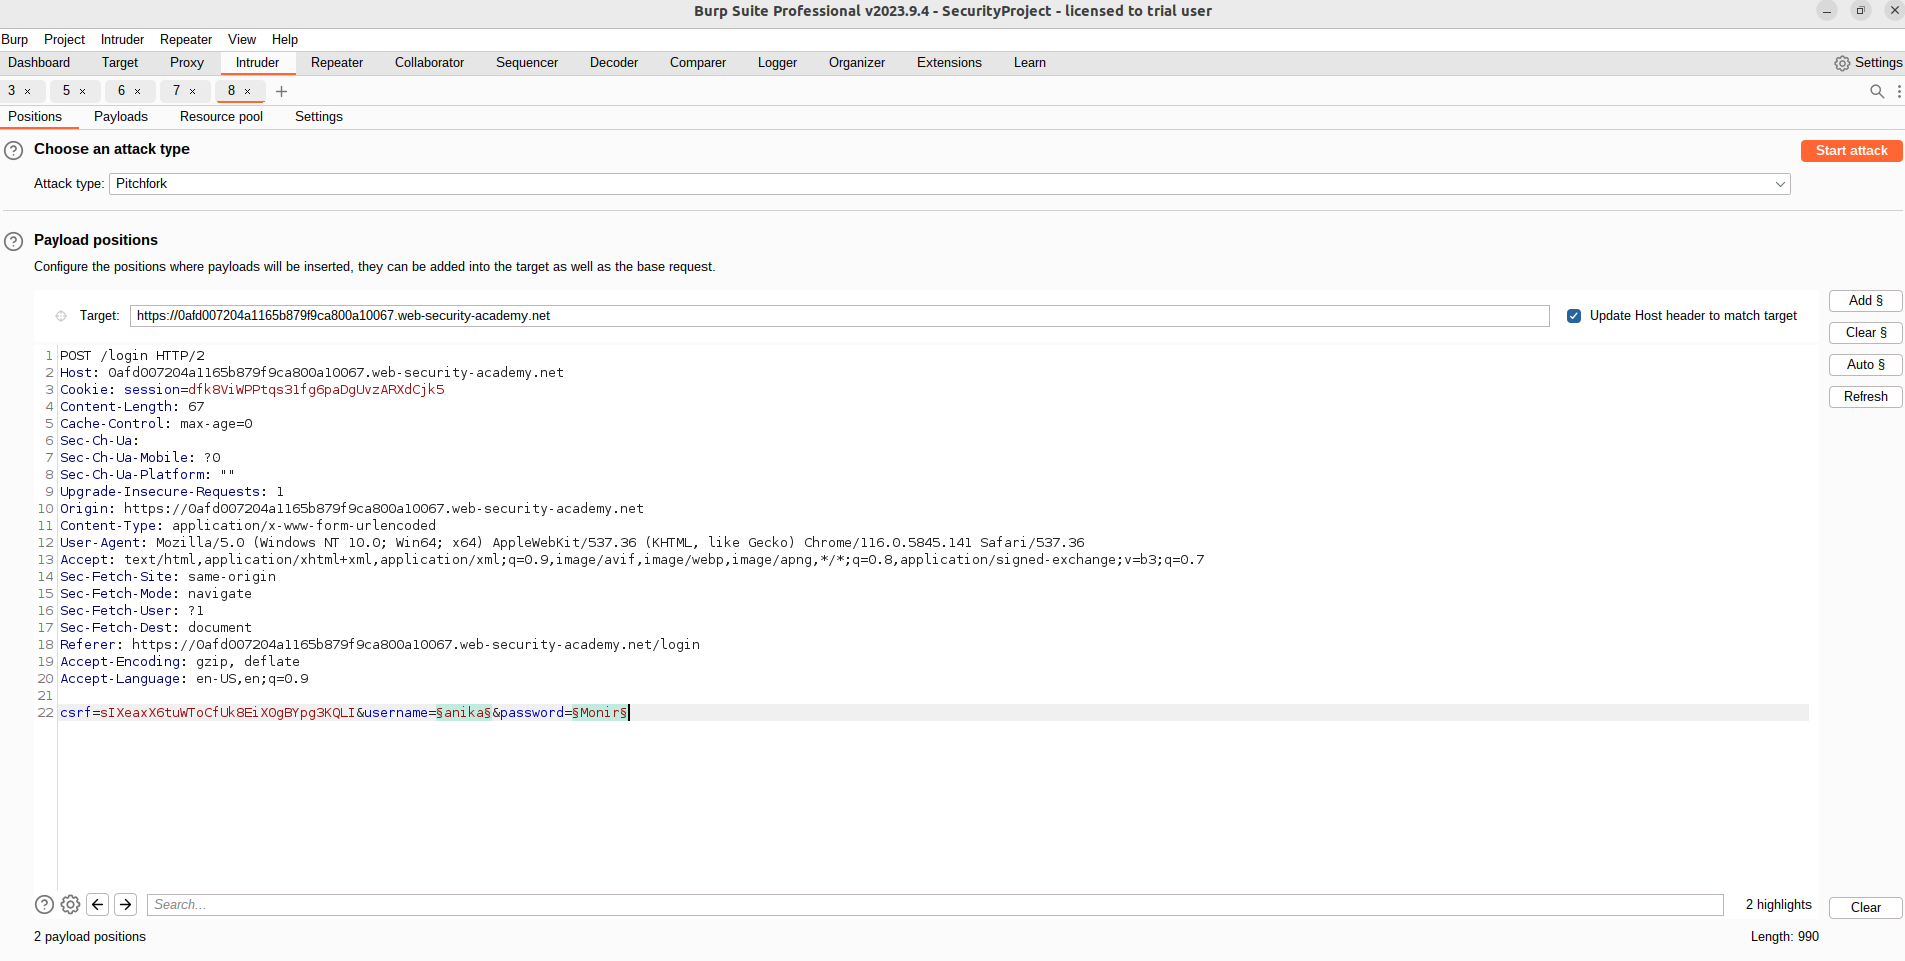
\includegraphics[width=1\textwidth]{Images/anikaScreensots/credentialStuffin1.png}
    \caption{setting the attack type as pitch fork }
    \label{fig:enter-label}
\end{figure}

 \begin{figure}[H]
    \centering
    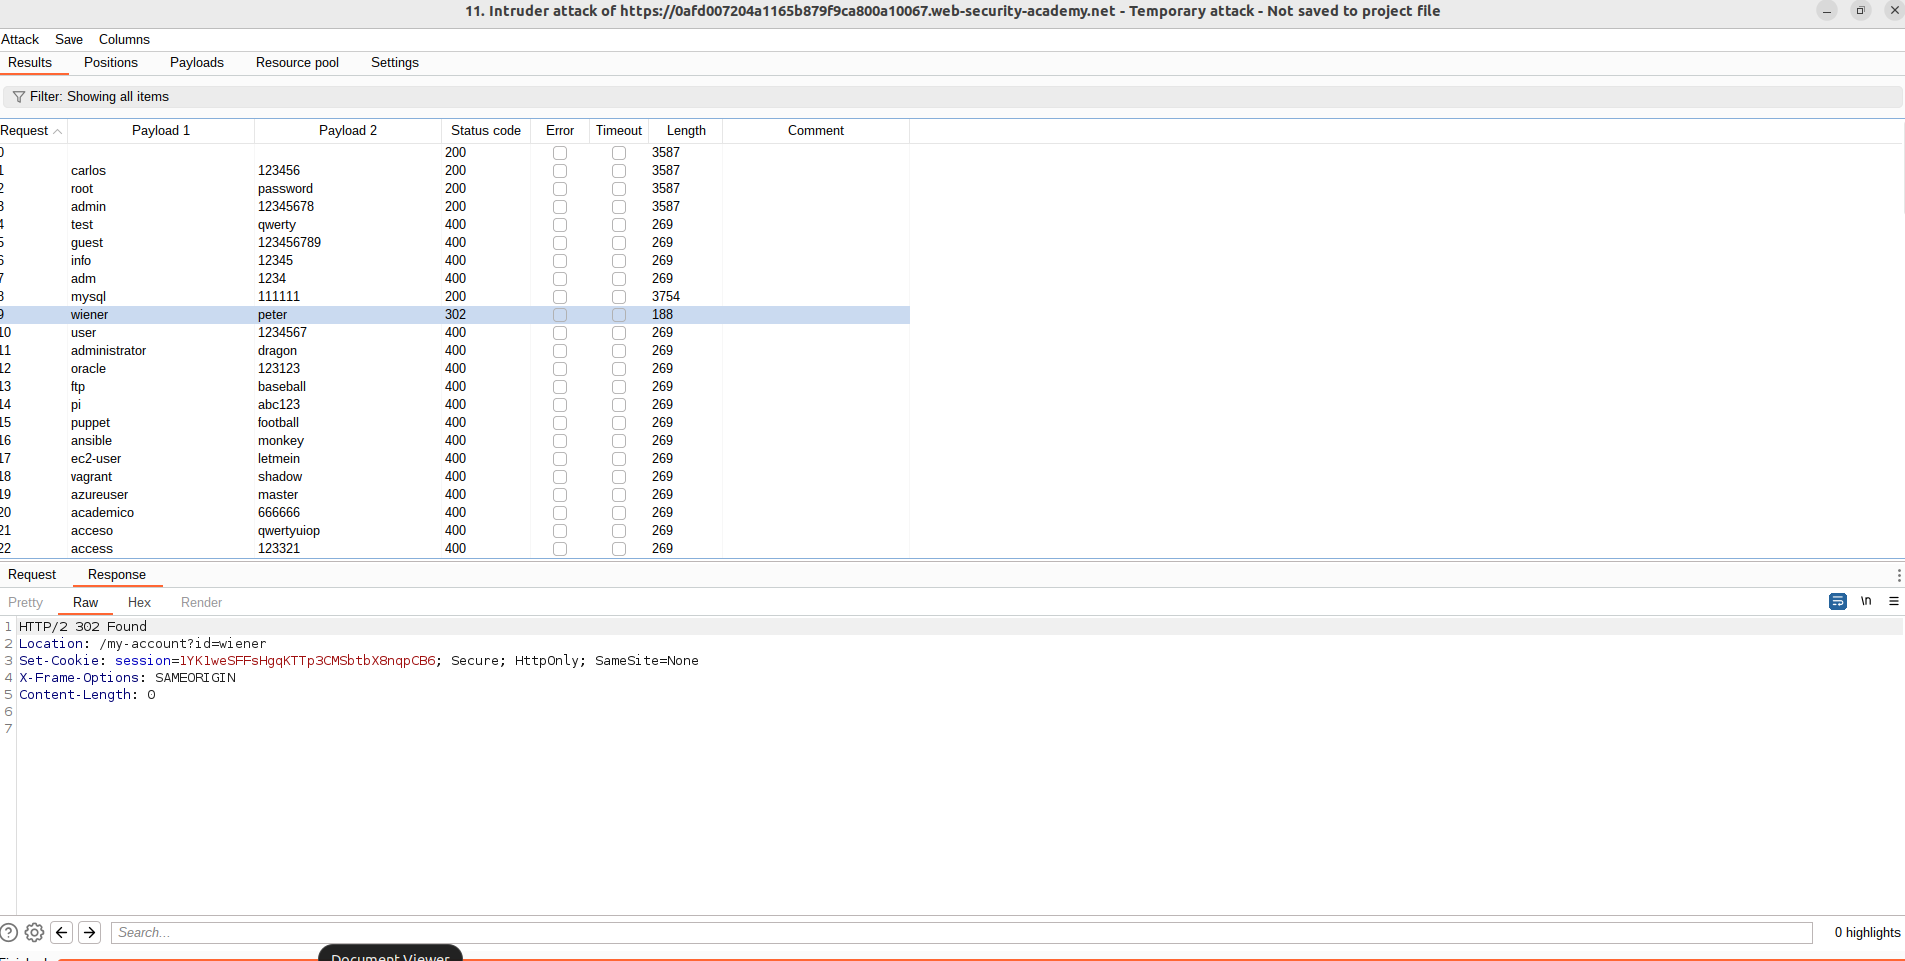
\includegraphics[width=1\textwidth]{Images/anikaScreensots/credentialStuff3.png}
    \caption{setting the payload as known password list from previous breaches}
    \label{fig:enter-label}
\end{figure}

 \begin{figure}[H]
    \centering
    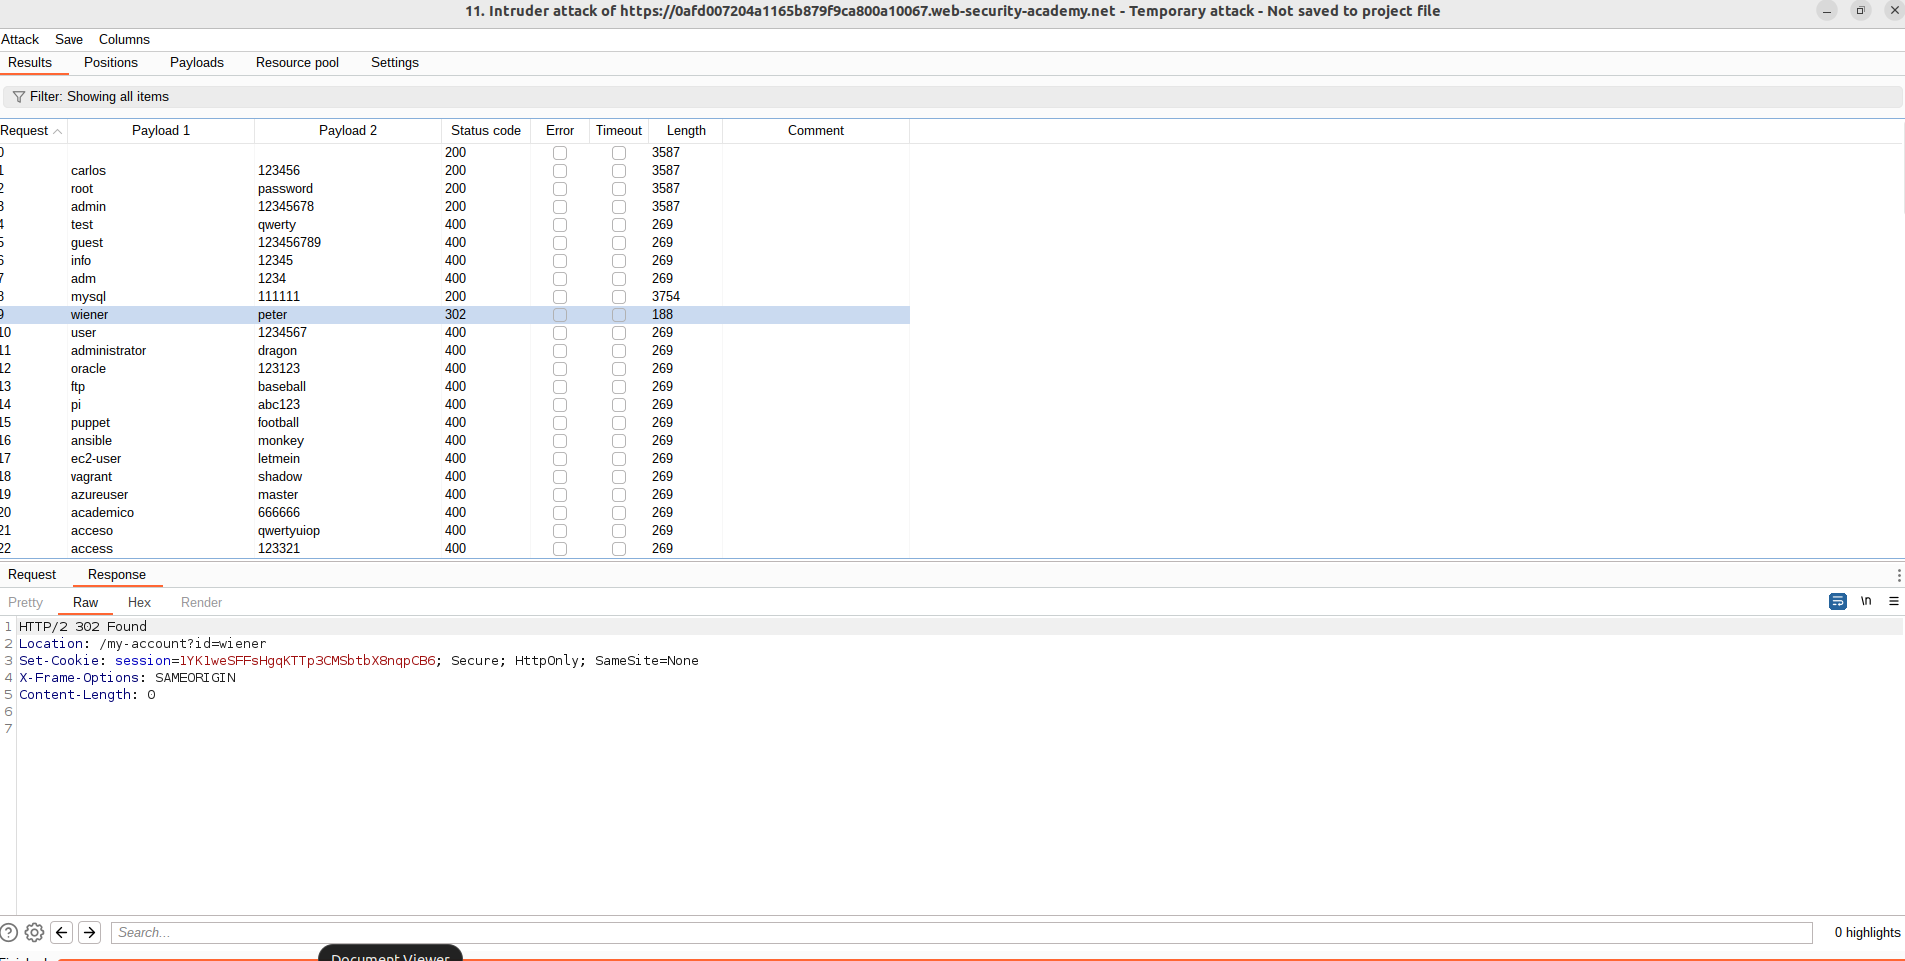
\includegraphics[width=1\textwidth]{Images/anikaScreensots/credentialStuff3.png}
    \caption{checking the response for each request and check for anomalies to gain knowledge}
    \label{fig:enter-label}
\end{figure}
 

\end{fullwidth}
\subsection*{Brute force login}

\begin{fullwidth}
    Since we may not always have any information on usernames and passwords- we can also brute force attacks using the cluster bomb attack type of intruder tool.


     \begin{figure}[H]
    \centering
    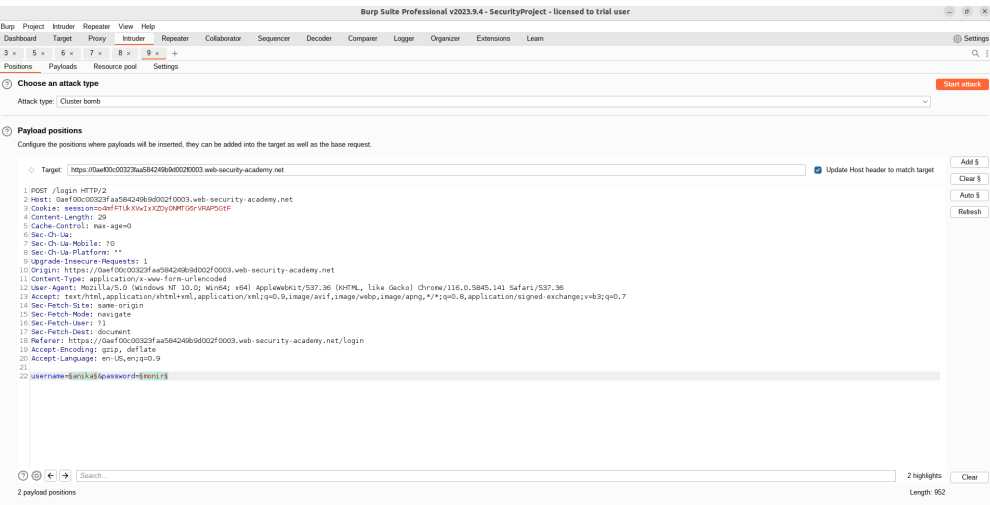
\includegraphics[width=1\textwidth]{Images/anikaScreensots/BruteForce1.png}
    \caption{setting the attack type as pitch fork}
    \label{fig:enter-label}
\end{figure}

 \begin{figure}[H]
    \centering
    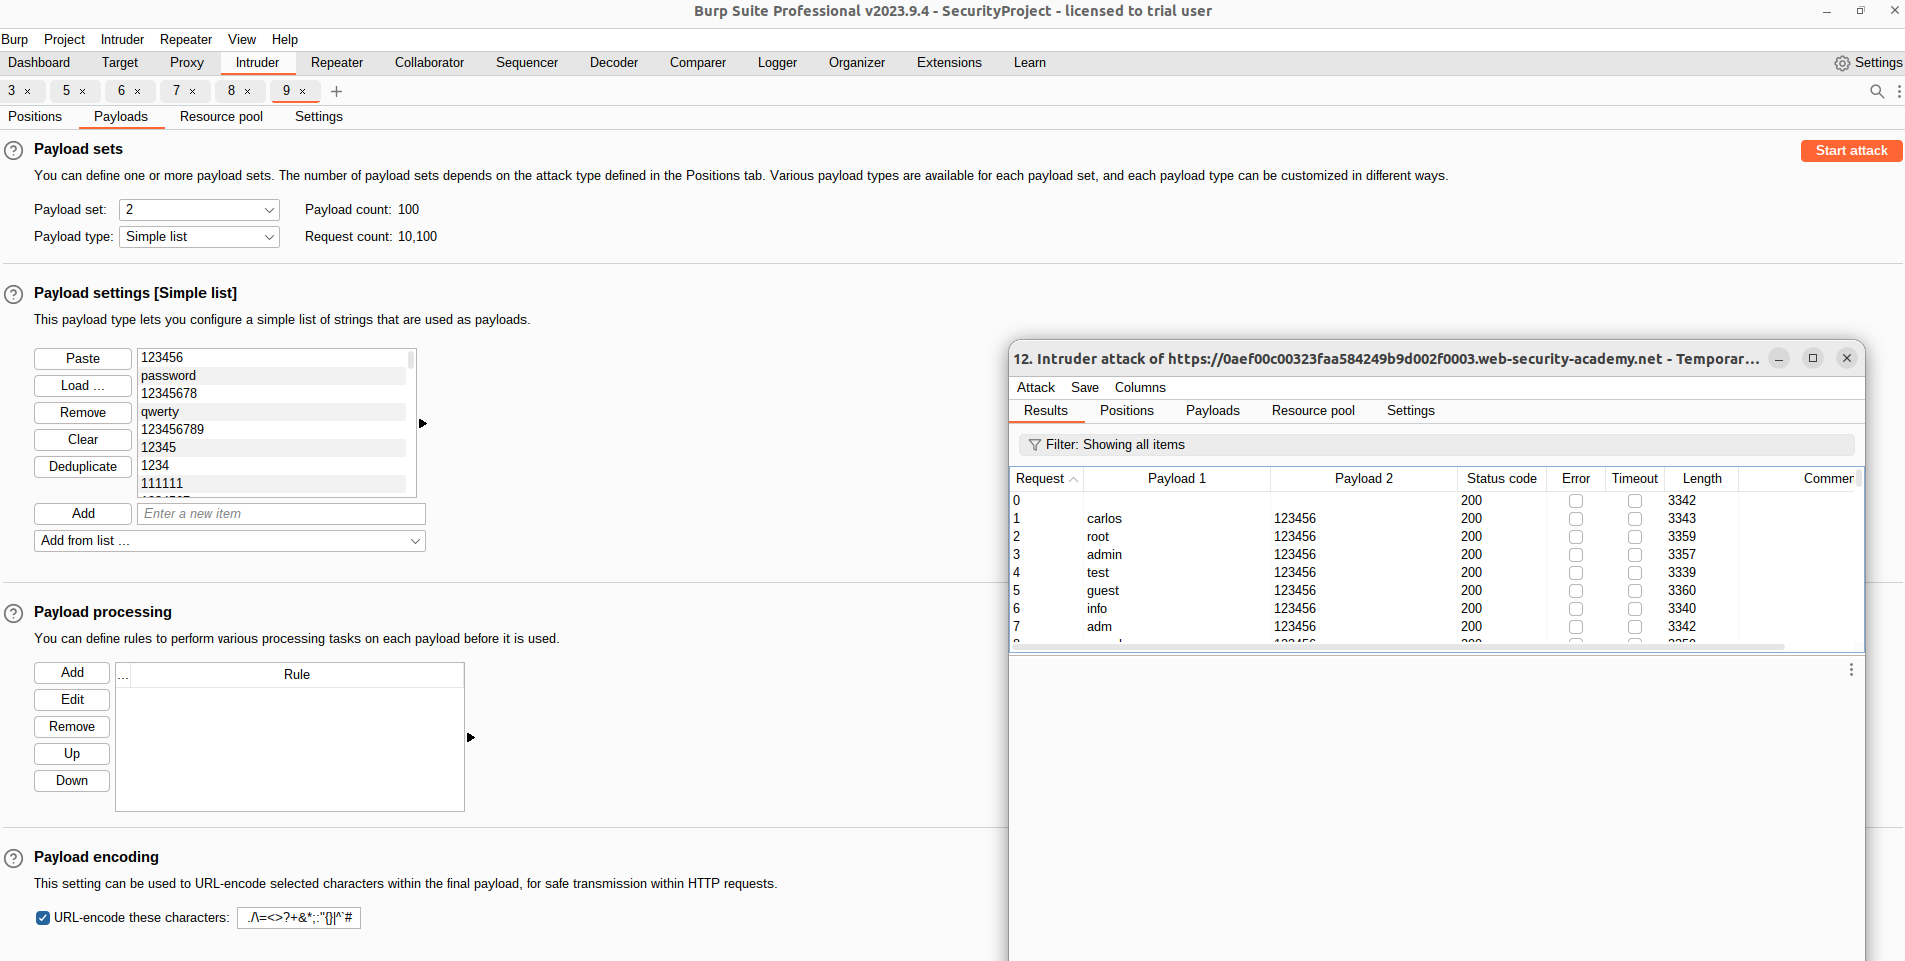
\includegraphics[width=1\textwidth]{Images/anikaScreensots/bruteForce2.png}
    \caption{setting the payload as known password list from previous breaches}
    \label{fig:enter-label}
\end{figure}

 \begin{figure}[H]
    \centering
    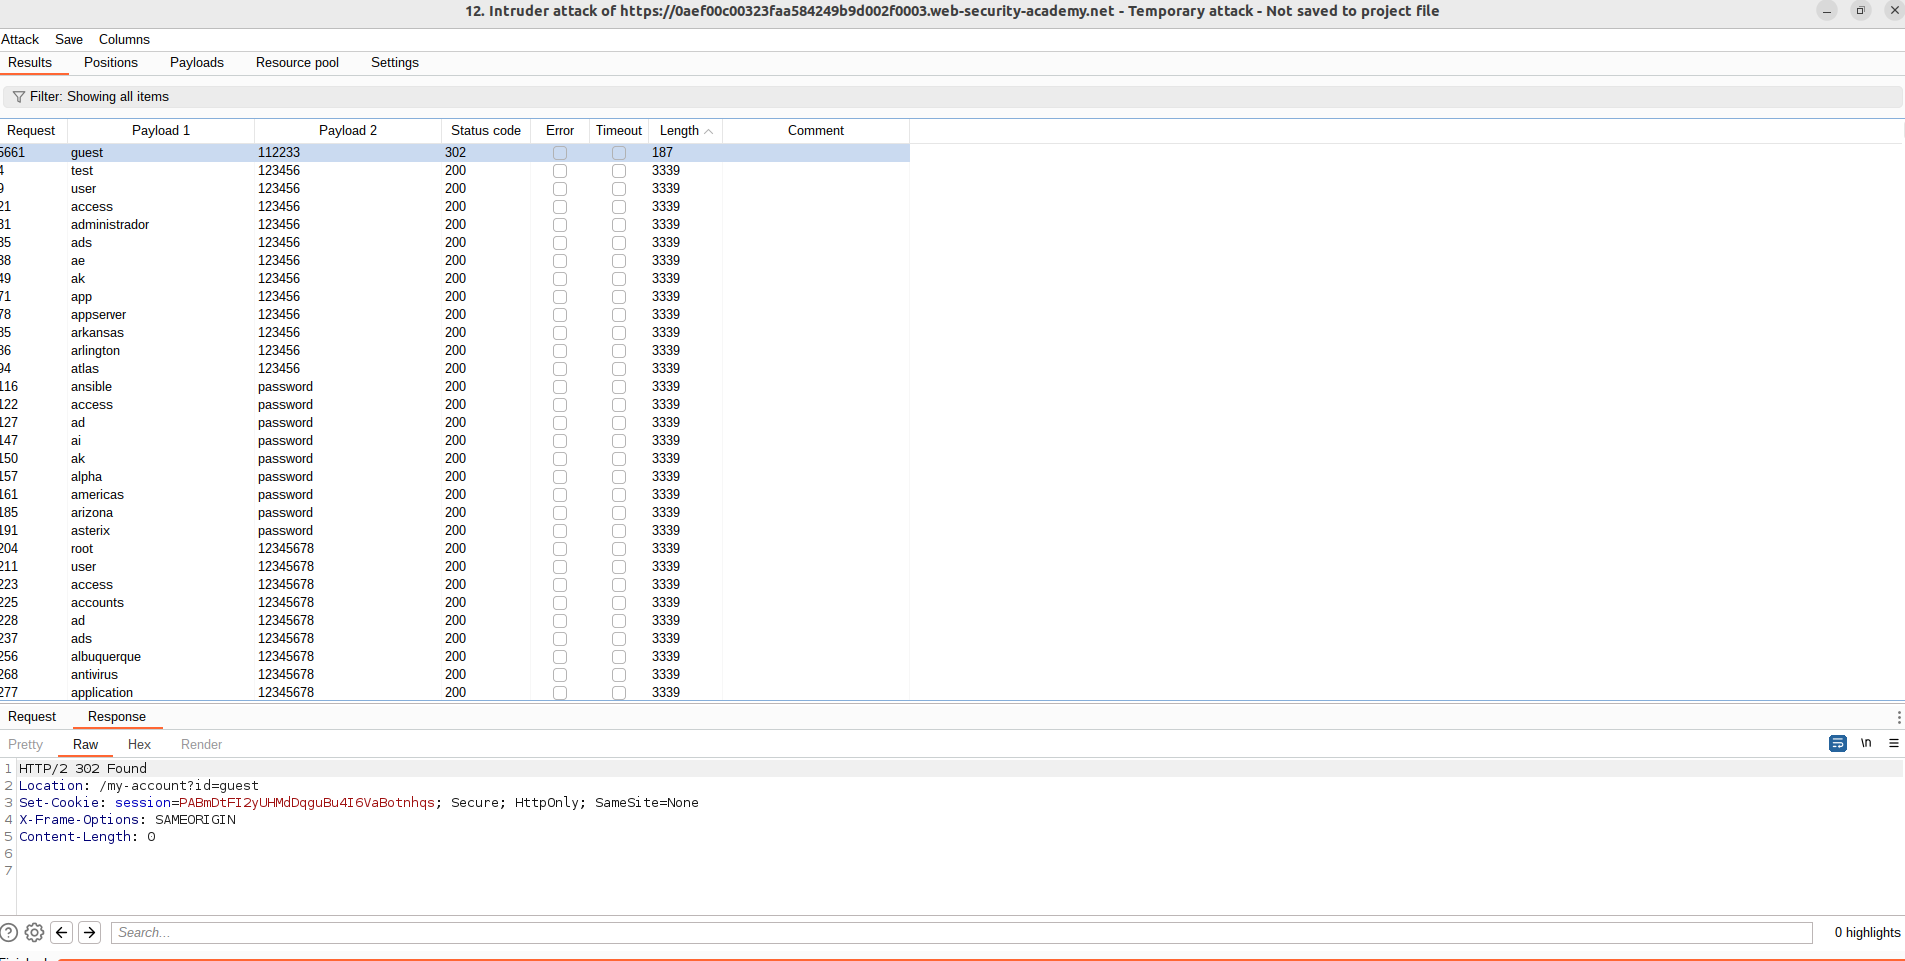
\includegraphics[width=1\textwidth]{Images/anikaScreensots/bruteForce3.png}
    \caption{checking the response for each request and check for anomalies to gain knowledge}
    \label{fig:enter-label}
\end{figure}

\end{fullwidth}
\subsection*{Privilege escalation}
\begin{fullwidth}
    
When a user logs in to an application, they usually only have access to the parts of the application that they need to perform their specific tasks. If access controls are incorrectly set, a user can gain access to functionality that should only be available to higher-privileged users.


\begin{figure}[H]
    \centering
    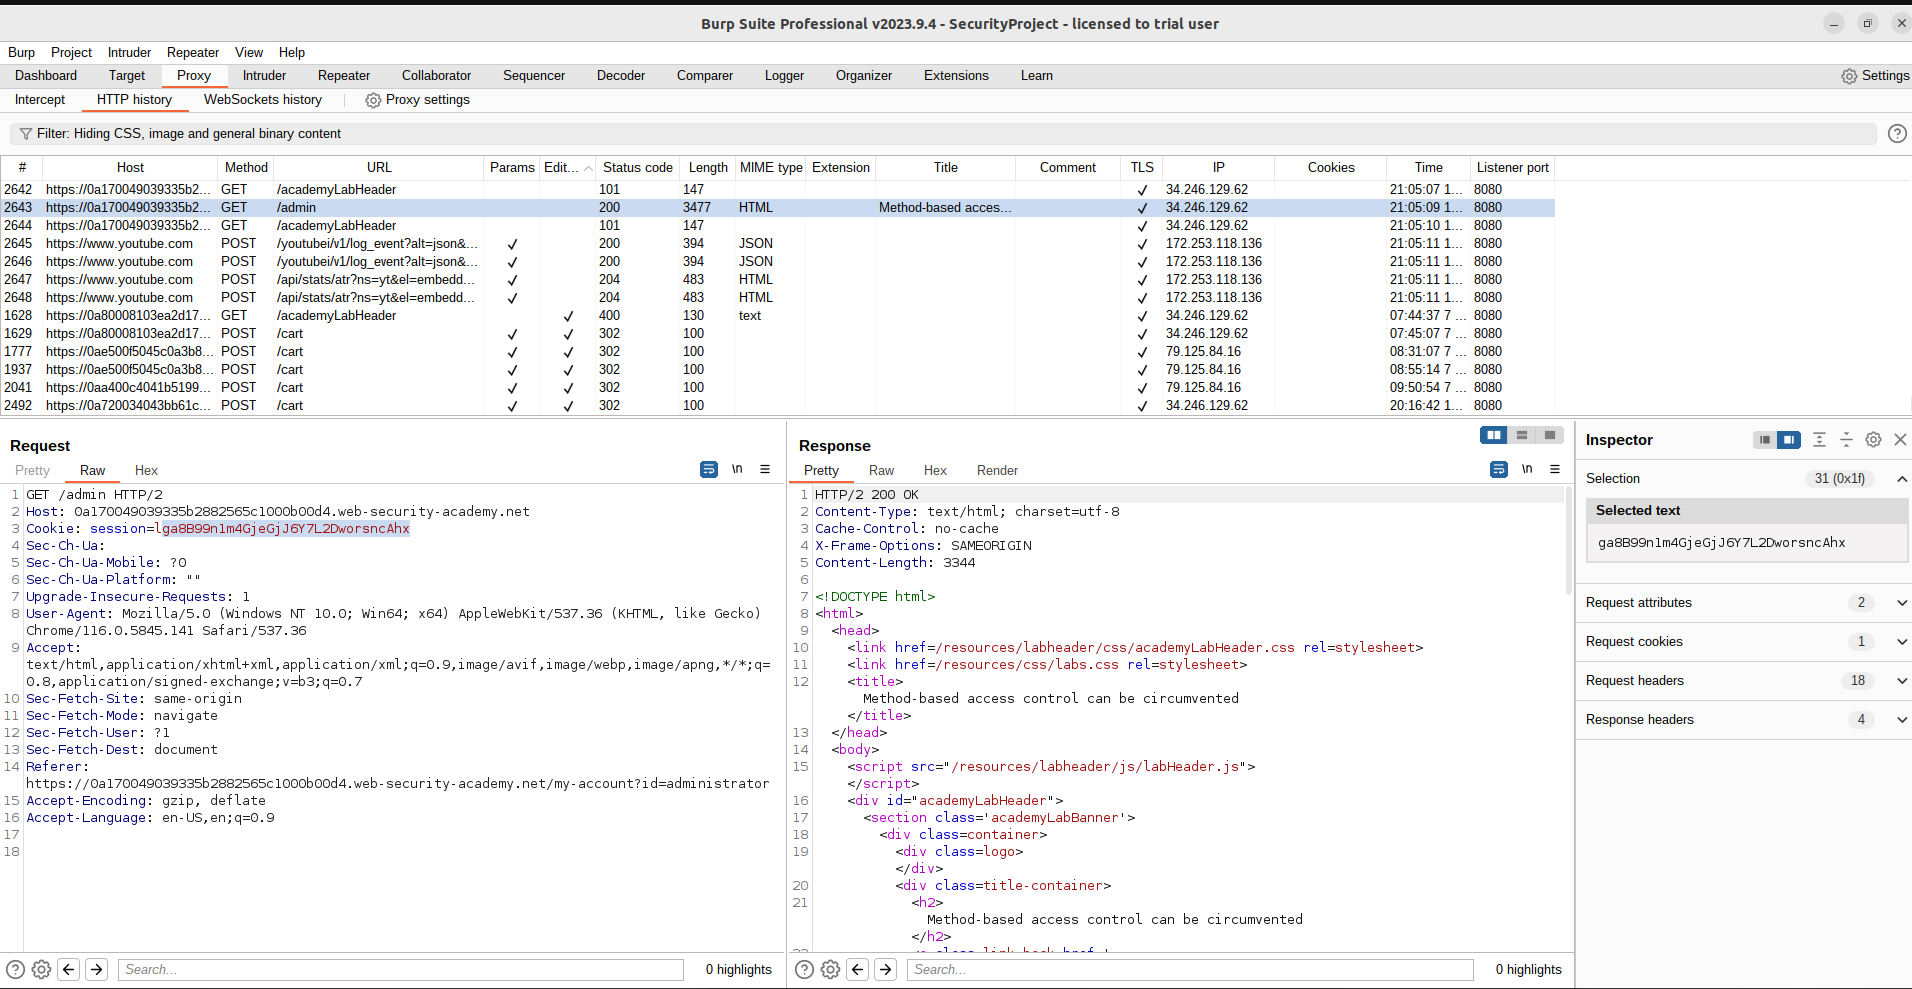
\includegraphics[width=1\textwidth]{Images/anikaScreensots/prev1.png}
    \caption{log in as an administrator and access the admin panel}
    \label{fig:enter-label}
\end{figure}


\begin{figure}[H]
    \centering
    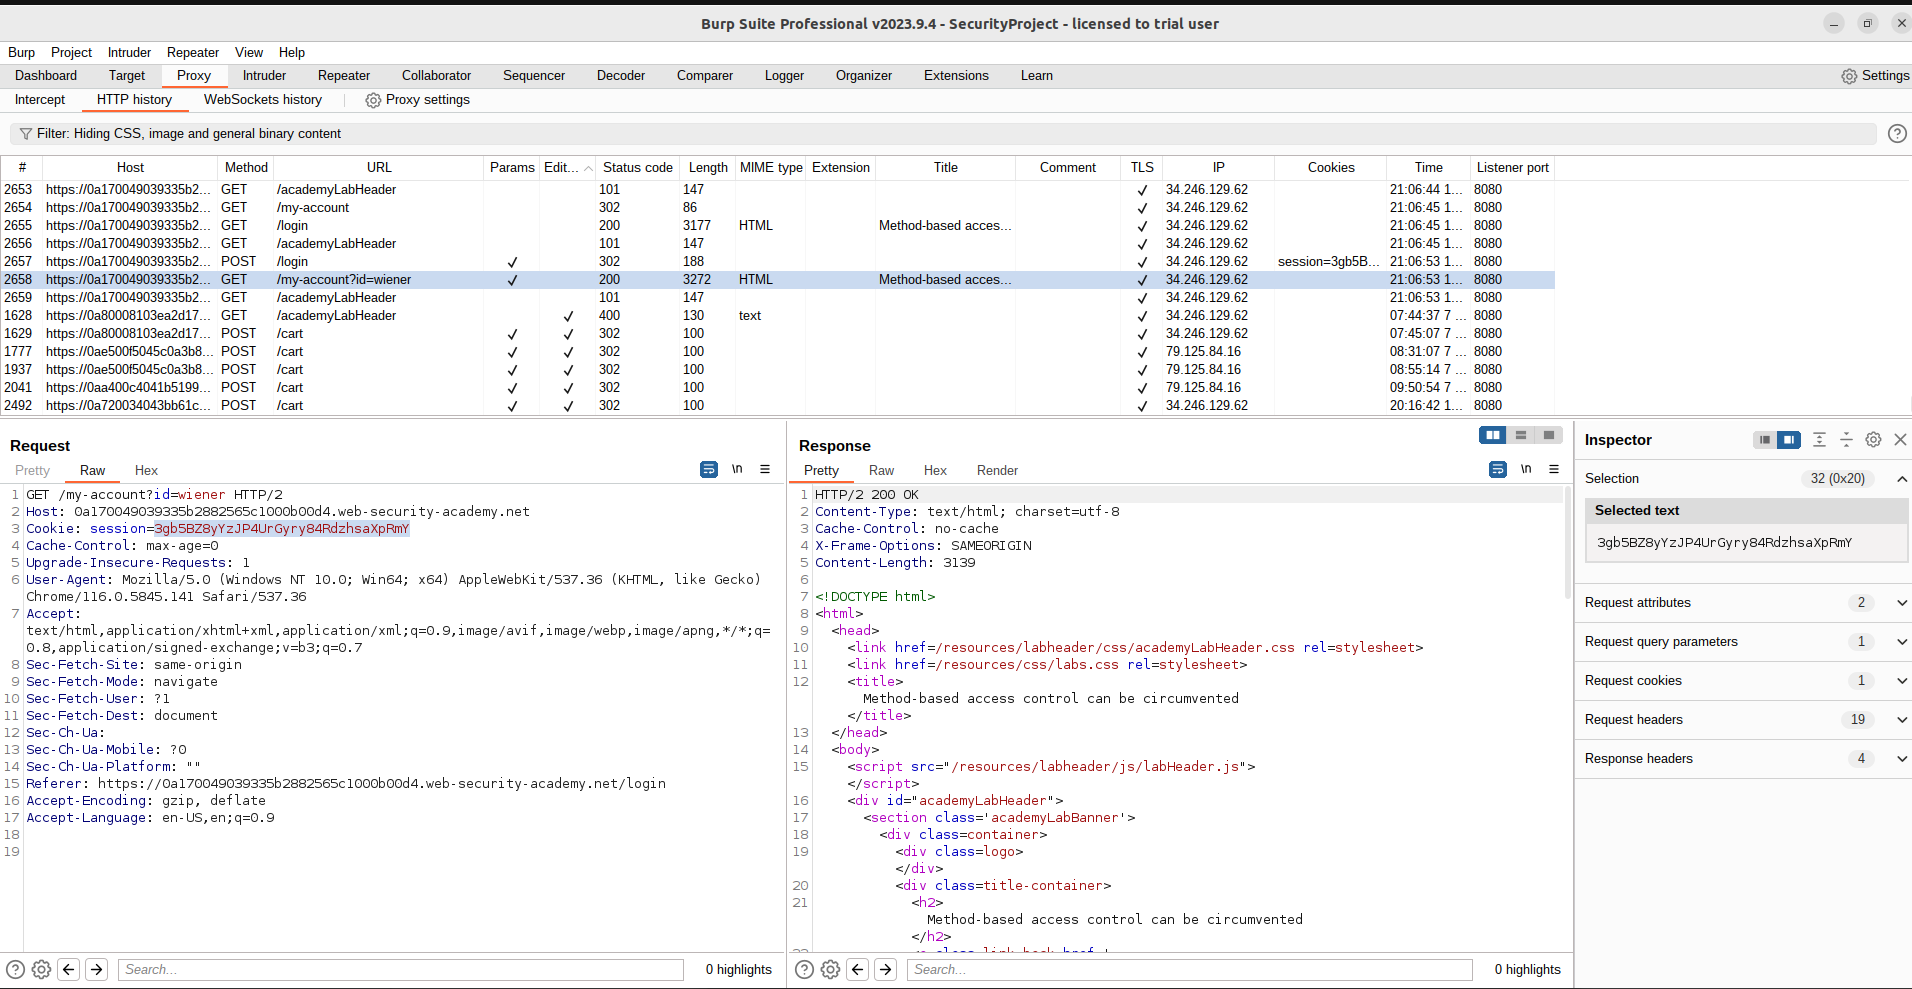
\includegraphics[width=1\textwidth]{Images/anikaScreensots/prev2.png}
    
    \caption{login as a normal user}
    \label{fig:enter-label}
\end{figure}

\begin{figure}[H]
    \centering
    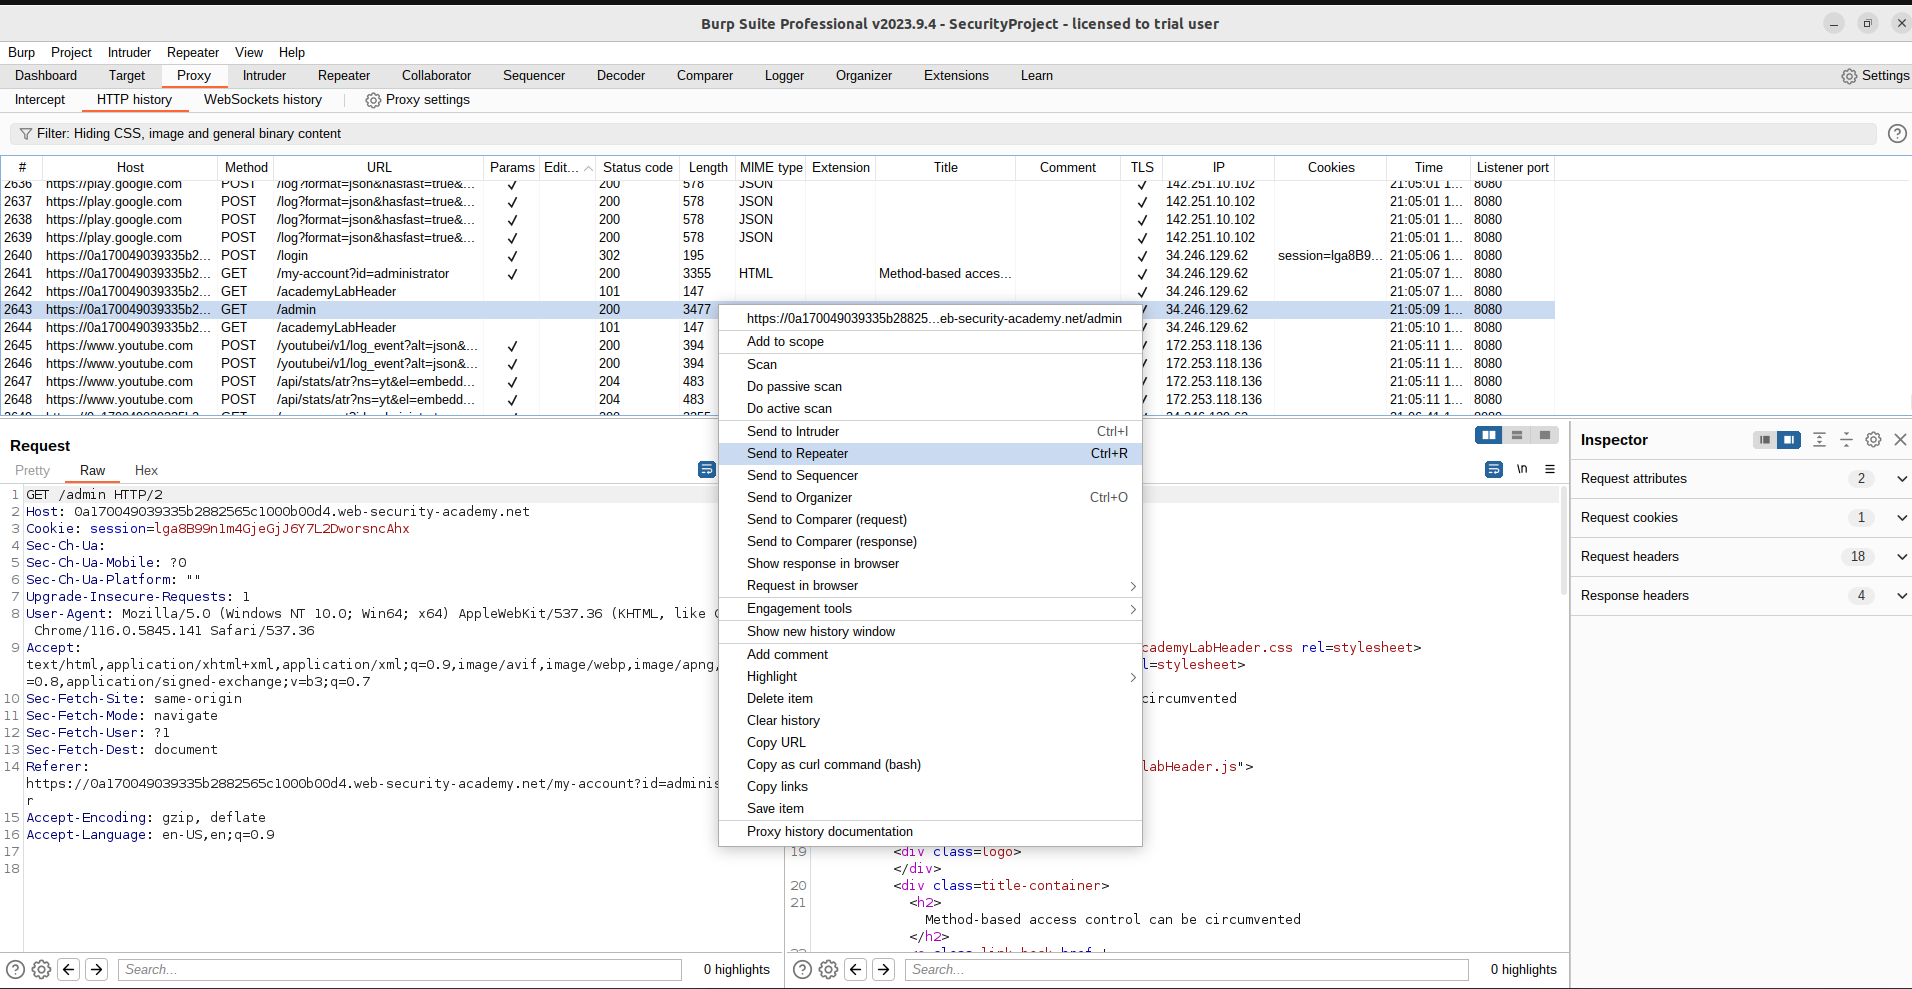
\includegraphics[width=1\textwidth]{Images/anikaScreensots/prev3.png}
    \caption{send the recent request of normal user to repeater}
    \label{fig:enter-label}
\end{figure}

\begin{figure}[H]
    \centering
    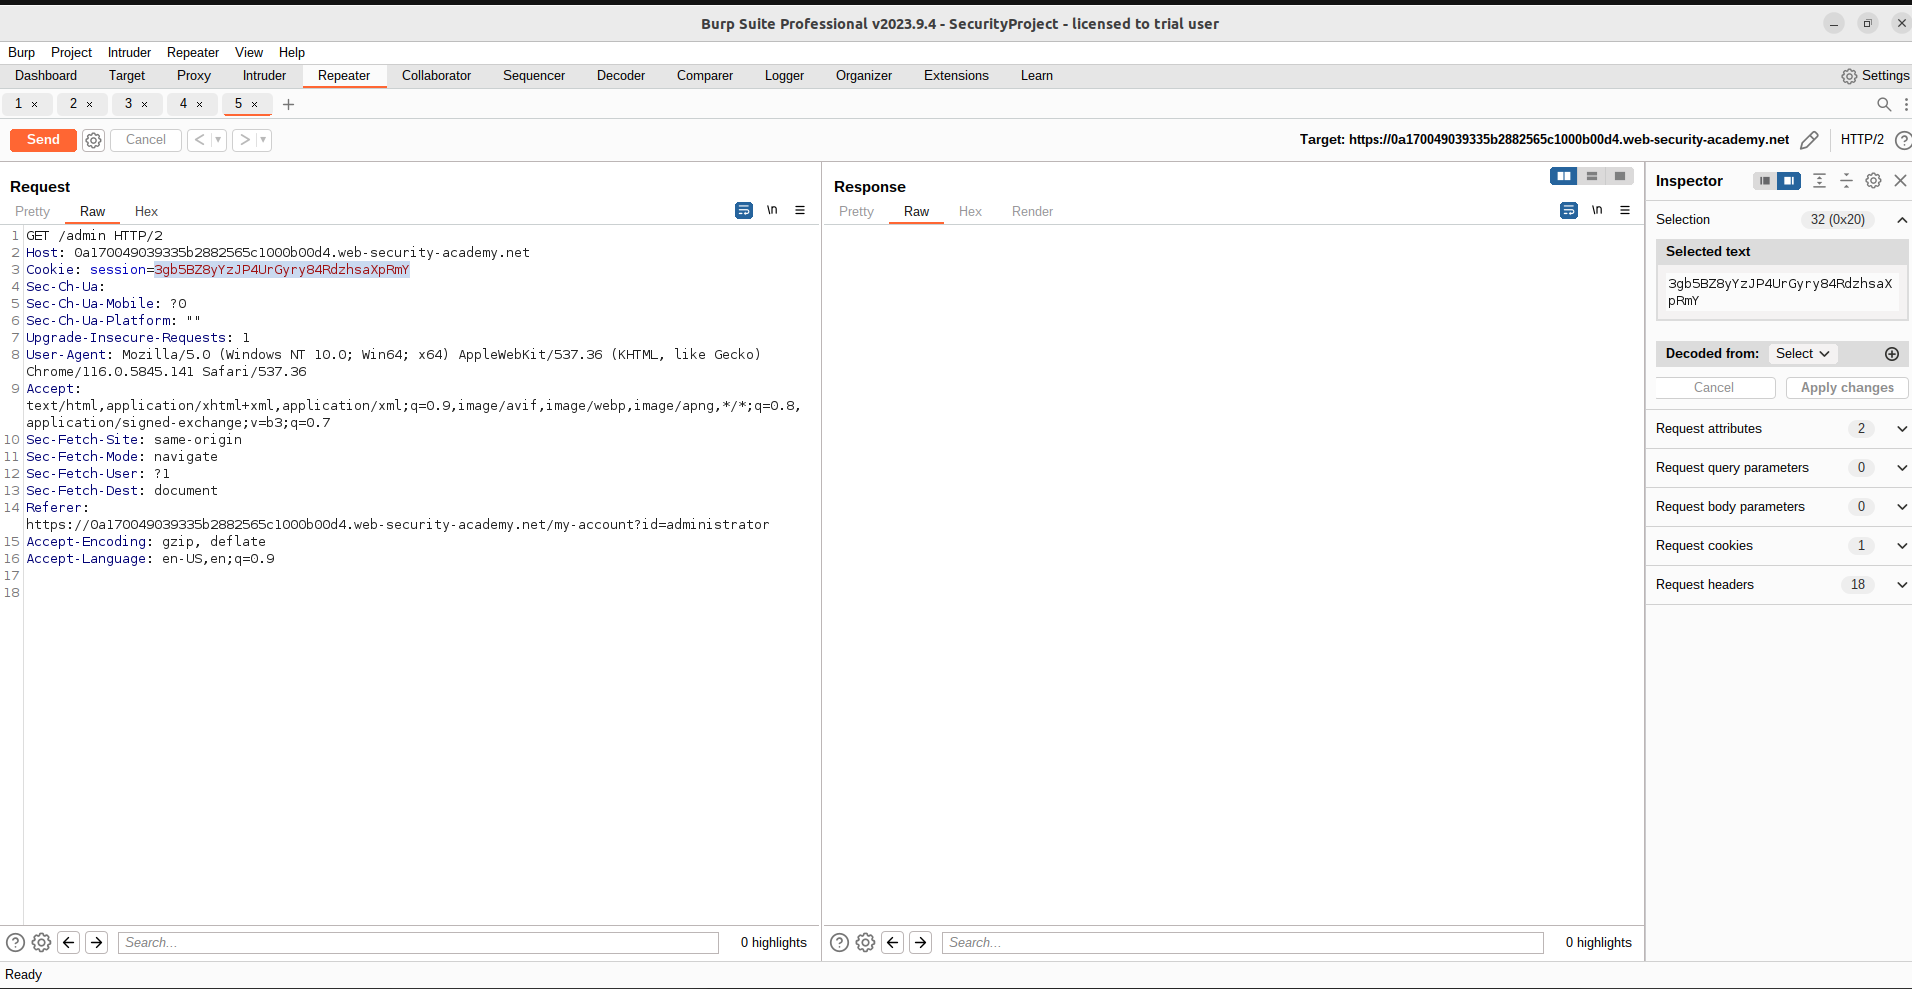
\includegraphics[width=1\textwidth]{Images/anikaScreensots/prev4.png}
    \caption{copy the session cookie of normal user to the administrative user}
    \label{fig:enter-label}
\end{figure}


\begin{figure}[H]
    \centering
    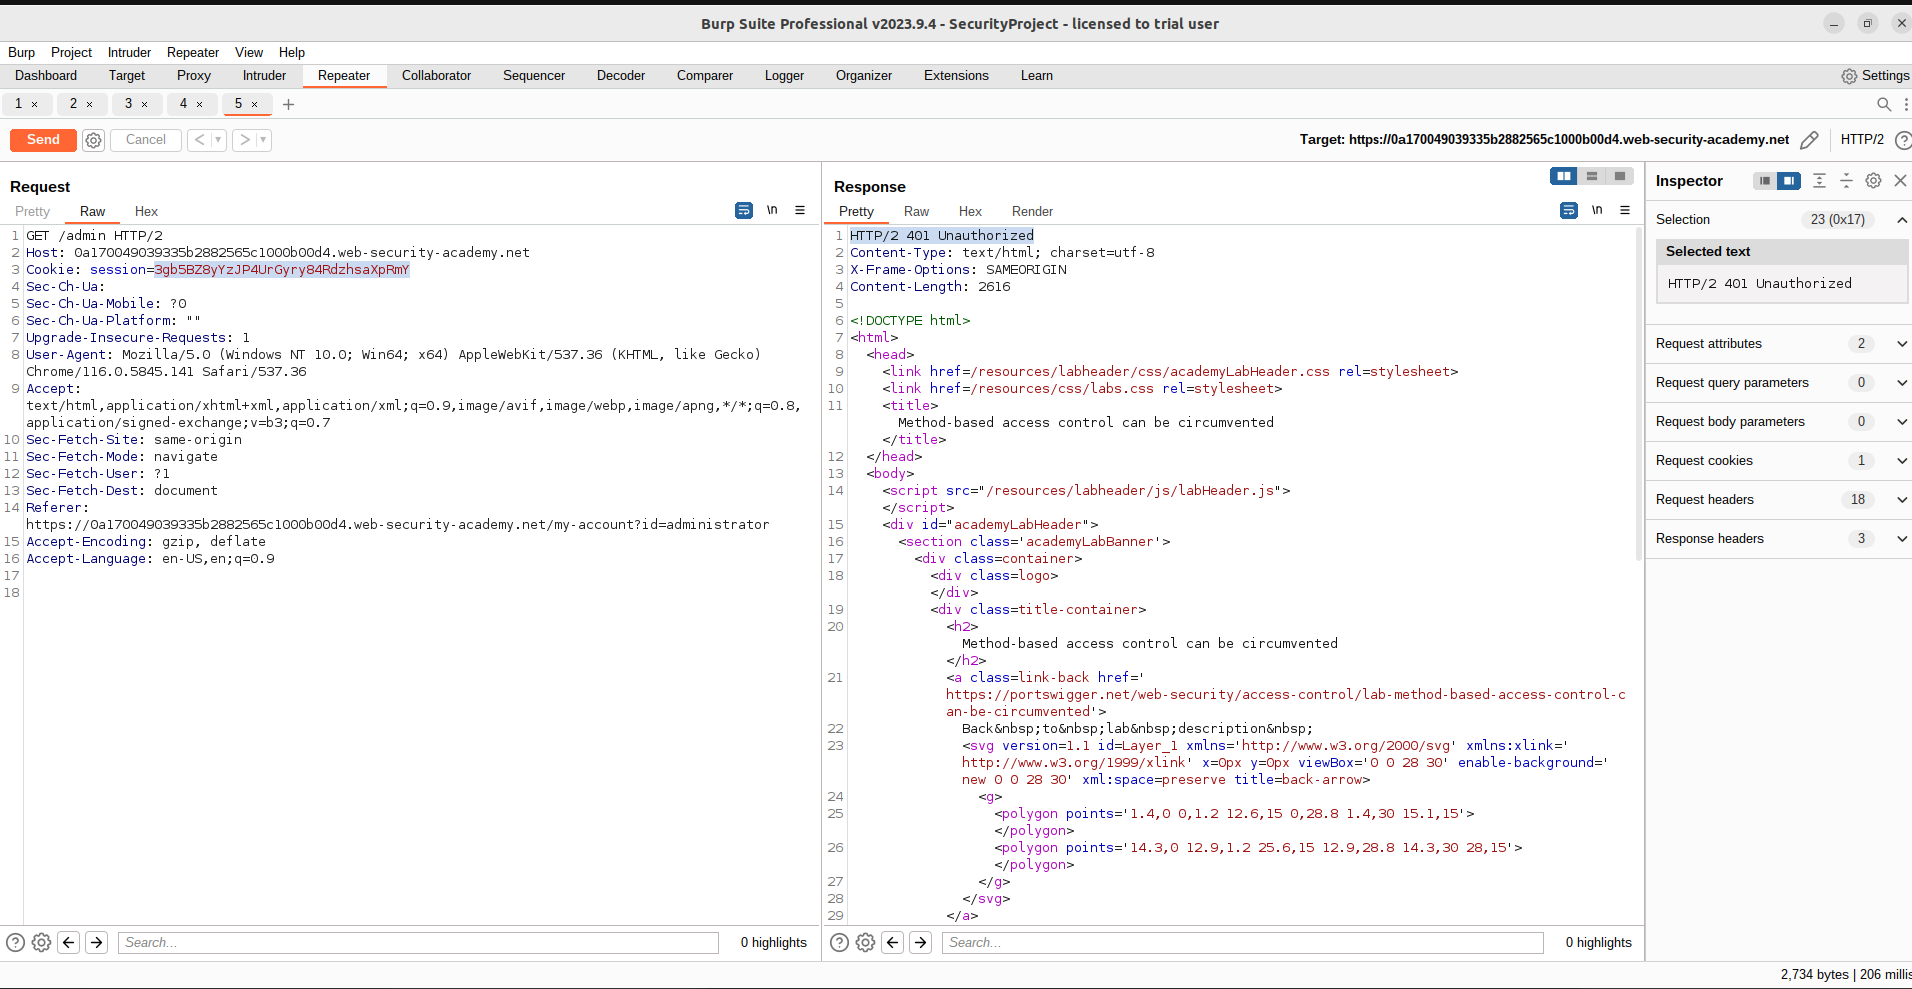
\includegraphics[width=1\textwidth]{Images/anikaScreensots/prev5.png}
    \caption{send the request and check if the security breach works.Here we got a 401 confirming that the endpoint is not vulnerable}
    \label{fig:enter-label}
\end{figure}

\end{fullwidth}


\end{document}
